
%%%%%%%%%%%%%%%%%%%%%%%%%%%%%%%%%%%%%%%%%%%%%%%%%%%%%%%%%%%%%%%%%%%%%%
% How to use writeLaTeX: 
%
% You edit the source code here on the left, and the preview on the
% right shows you the result within a few seconds.
%
% Bookmark this page and share the URL with your co-authors. They can
% edit at the same time!
%
% You can upload figures, bibliographies, custom classes and
% styles using the files menu.
%
%%%%%%%%%%%%%%%%%%%%%%%%%%%%%%%%%%%%%%%%%%%%%%%%%%%%%%%%%%%%%%%%%%%%%%

\documentclass[12pt]{article}

\usepackage{sbc-template}
\usepackage[square,sort,comma,numbers]{natbib}
\usepackage{amsmath}
\usepackage{color,soul}
\usepackage{graphicx,url}
\usepackage{multicol}
\usepackage{diagbox}
\usepackage[dvipsnames]{xcolor}
\usepackage{verbatim}
\usepackage{makecell}

\newcommand{\R}[1]{~\scriptsize{(#1)}}
\newtheorem{definition}{Definition}

%\usepackage[brazil]{babel}   
\usepackage[utf8]{inputenc}  

     
\sloppy

\title{SMSM: a Multidimensioanl Similarity Measure for Trajectory Stops and Moves}

\author{Andre L. Lehmann\inst{1}, Luis Otavio Alvares\inst{1}, Vania Bogorny\inst{1} }


\address{Programa de Pós-Graduação em Ciência da Computação \\Departamento de Informatica e Estatistica, Universidade Federal de Santa Catarina\\ Florianopolis, Santa Catarina, Brasil
  \email{andre.lehmann@posgrad.ufsc.br,alvares@inf.ufsc.br ,vania.bogorny@ufsc.br}
}

\begin{document} 

\maketitle

\begin{abstract}
For many years trajectory similarity research has focused on raw trajectories, considering only space and time information. With the trajectory semantic enrichment emerged the need for similarity measures that support space, time, and semantics. Although some trajectory similarity measure deal with all three dimensions, they consider only stops or raw trajectories, ignoring the moves. We claim that, for some applications, the movement between stops is as important as the stops, and they must be considered in the similarity analysis.
  In this article we propose SMSM, a novel similarity measure for semantic trajectories that considers both stops and moves.
  SMSM is evaluated with real trajectory data of CRAWDAD and Geolife. The results show that SMSM overcomes state-of-art measures.
\end{abstract}

\section{Introduction}

Trajectory similarity measuring has received significant attention in the last few years, and several measures have been proposed {to deal either with raw trajectories or semantic trajectories}. A \emph{raw trajectory} is generally represented as a sequence of points $T=<p_1, p_2, ...p_n>$, with $p_i=(x_i,y_i,t_i)$ where $x,y$ is the position of the object in space at time instant $t$.  Examples of similarity measures for raw trajectories are LCSS (Longest Common SubSequence) \citep{vlachos2002discovering}, EDR (Edit Distance on Real sequences) \citep{Chen:2005:RFS:1066157.1066213}, NWED (Normalized Weighted Edit Distance) \citep{dodge2012} and UMS (Uncertain Movement Similarity) \citep{Furtado-UMS-2018}. LCSS \citep{vlachos2002discovering} and EDR \citep{Chen:2005:RFS:1066157.1066213} consider the sequence, but they force a match in all dimensions, not allowing partial similarity between trajectory points.  %{Multi-Dimensional Dynamic Time-Warping} (MD-DTW) \cite{ten2007multi} is another approach that is able to handle multiple dimensions. It extends {Dynamic Time-Warping} (DTW) \cite{berndt1994using} in order to find the distance between two sequences by looking for the best contiguous match of elements according to the sum of the distances in all dimensions. The problem of DTW and MD-DTW is that they consider the real distance between the elements, are sensitive to noise, and were developed for numerical attributes, not dealing with semantic information. 
UMS \citep{Furtado-UMS-2018} is a parameter free method that considers only the spatial dimension, but it outperformed all previous works for raw trajectory similarity.


Existing works for raw trajectory similarity are limited to the spatio-temporal properties of raw trajectories, basically considering trajectories as objects with only space information or space and time.

In 2008, emerged the concept of semantic trajectories \citep{Spaccapietra:2008:CVT:1347466.1347785}, where trajectories are represented as \emph{sequences of stops and moves}. \emph{Stops} are the most important parts of trajectories, representing the places that an object has visited for a minimal amount of time, and the \emph{moves} are the trajectory points between stops. In several works, stops are called points of interest (POIs), episodes, or stay points. Semantic trajectories are more complex than raw trajectories, because they have at least three dimensions: space, time, and semantics. {We consider in this paper that semantics is any type of information associated to mobility data other than spatial location and time.}

{The enrichment of trajectories with semantic information is a well studied topic in the literature, and a number of methods have been proposed for this purpose, as the works of} \cite{alvares2007model}, \cite{Palma2008}, \cite{manso}, and \cite{fileto2013baquara}. {Examples of semantic information related to the stops can be, for instance, the name of the stop (e.g. Ibis Hotel) and the category (e.g. Hotel, Museum, Restaurant), while the semantic information related to the move could be, for instance, the name of the streets followed by the moving object and the category of the transportation mode. The explosion of social media data, internet channels, and the facility to enrich trajectories with more context information as linked open data, allows the representation of movement in a more meaningful way. From social media data, for instance, a stop at a hotel can be enriched with the information of the number of stars, the price average, evaluation rate, facilities, parking, wifi, etc.  In this paper we assume that semantic trajectories are represented as sequences of stops and moves, as originally defined in }\cite{Spaccapietra:2008:CVT:1347466.1347785}{, and the way how these trajectories are generated or enriched is out of the scope of this paper.}

{Only a few  similarity measures were proposed for semantic trajectories, as } \cite{Kang:2009:SMT:1529282.1529580}, \cite{Liu:2012:SMM:2442968.2442971}, \cite{Ying:2010:MUS:1867699.1867703}, and \cite{Furtado:TGIS12156}{. The main problems of these measures are that they do not address all three dimensions (space, time and semantics), as the works of }\cite{Kang:2009:SMT:1529282.1529580} and \cite{Liu:2012:SMM:2442968.2442971}{; or, 
they exclusively address the stops, systematically ignoring all information about the moves, as the works of }\cite{Ying:2010:MUS:1867699.1867703} and \cite{Furtado:TGIS12156}{. To the best of our knowledge, none of the existing similarity measures for semantic trajectories have considered both stops and moves. The measure MSM (Multidimensional Similarity Measure) }\citep{Furtado:TGIS12156}{, for instance, considers only the stops, and they are treated as elements that are independent from each other, without considering the order/sequence as they appear in the trajectories. However, MSM ignores the moves between stops. MSM can be used to answer questions like: \emph{how similar are two trajectories $P$ and $Q$ considering their stops?}}
%In the example shown in Figure {\ref{fig:Paris}}, that shows the trajectories of three tourists visiting the same places (stops S1, S2, S3 and S4) in Paris, MSM would give a similarity degree of 100\%, because the objects visited the same places and MSM ignores the moves.

 

{Similarity measures are the basis of several data processing and analysis techniques, such as information retrieval, location prediction, nearest neighbour queries, outlier detection, clustering, etc. A clustering algorithm, for instance, uses a similarity measure for grouping objects with similar trajectories. Outlier detection methods use similarity to find groups of trajectories with normal behavior, and the objects that are dissimilar to the majority, are the outliers. To detect specific trajectory patterns such as flocks }\citep{Laube2005}{, for instance, a raw trajectory similarity measure could be applied to find a minimal number of objects moving together in space and time. Similarity measures that consider both stops and moves can be important in a vast number of applications such as public transportation systems, traffic management, fraud detection, tourism, urban planning, etc. }
%To mention a few examples, similarity measures are the basis for finding objects that follow the same routes, tourists that visit similar places at similar times, to distinguish categories of users such as students from professors at a university, to find similar taxi trajectories, to find users that use the same means of transportation when visiting the same places, etc.


\begin{figure}[h]
\label{fig:Paris}
\centering
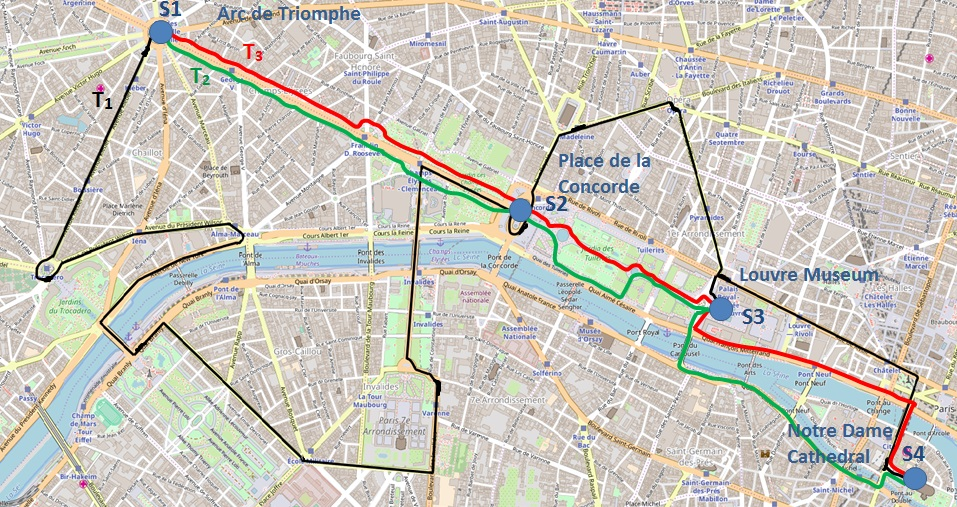
\includegraphics[width=1.0\textwidth]{Images/paris5.jpg}
\caption{Tourist trajectories in Paris with four stops}
\end{figure}


{To better understand the need for considering both stops and moves in trajectory similarity analysis, let us consider the example in Figure {\ref{fig:Paris}}, for a tourism application, which shows three trajectories of tourists visiting Paris. These tourists visited four places, in this order:  Arc de Triomphe (first stop - S1), Place de la Concorde (second stop - S2), the Louvre Museum (third stop - S3), and the Notre Dame Cathedral (the last stop - S4). The three tourists visited the same places at the same order, but the tourists of trajectories $T2$ (green trajectory) and $T3$ (red trajectory) moved on foot, following the shortest path, while the tourist of trajectory $T1$ used a city tour hop on and hop off bus to appreciate the view. From the figure it is clear that trajectories $T2$ and $T3$ are more similar, because they used almost the same paths between stops and moved on foot, while trajectory $T1$ has a completely different move. Now suppose that a tourism manager wants to recommend a trip to a new tourist arriving in Paris, and this new tourist wants to visit the same places visited by the tourists in the figure, but he wants to move on foot and follow the path used by the majority of the tourists.
For this case, we need to retrieve trajectories $T2$ and $T3$. 
%Another example is to calculate the proportion of tourists that visit these four stops moving on foot in order to eventually propose a new hop on hop off tourist bus line.
Another example is the evaluation of the flow of tourists moving on foot between these four stops in order to eventually propose a new and direct hop on hop off tourist bus line.}
%Another example is a tourism manager that wants to send advertisements for pedestrians about a new restaurant at Champs Elysées Avenue between \emph{Arch de Triomphe} and \emph{Place de la Concorde}.}
%From the whole database of trajectories, a query must return the most similar trajectories to the trajectory that this new user wants to perform. It is clear that for this problem, a good recommendation is only possible if we consider the sequence of visited places, the duration of the visits, the real path followed during the move, as well as the move transportation mode. 

{In taxi fraud detection, for instance, a similarity measure will help to answer questions like: given two regions of interest, which is the standard path followed by the majority of the taxis and which are the outliers?
%to find a taxi fraud trajectory between two given stops, a similarity measure must be used to find the standard path that connects the stops, for then identifying the outlier trajectories. 
A real example of an outlier taxi trajectory is shown in Figure {\ref{fig:crawdad_outlier}}, in the San Francisco dataset of the Crawdad project} \citep{epfl-mobility-20090224}. {In this example, given the stops Airport and  Westfield San Francisco Centre (WSFC), a similarity measure must consider both stops and moves to find the black trajectories as the most similar movements between the Airport and WSFC, and the trajectory in purple as the most dissimilar trajectory, which made a completely different and longer trip.}
 
\begin{figure}[h]
\centering
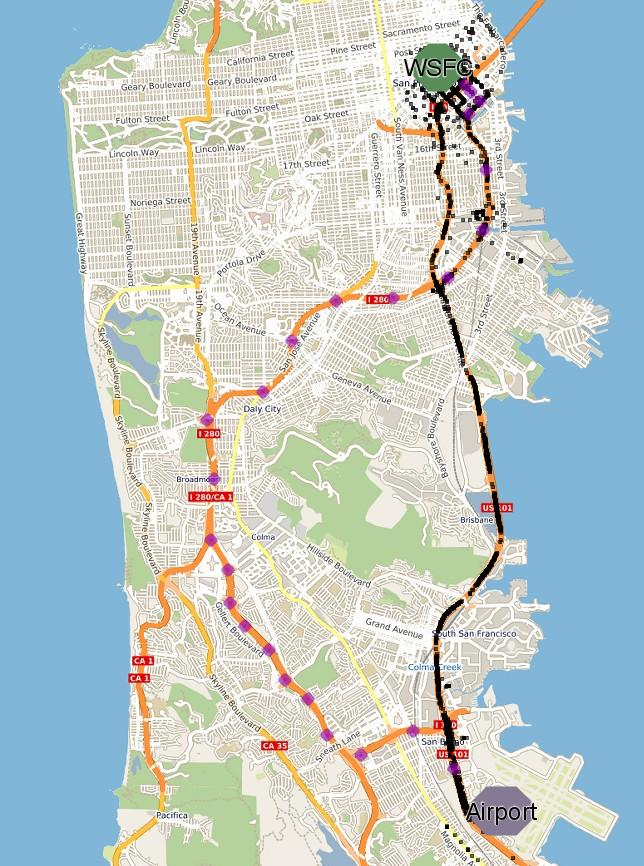
\includegraphics[width=0.5\textwidth]{Images/CRAWDAD-Outlier.jpg}
\caption{\label{fig:crawdad_outlier} An outlier trajectory (in purple) going from Airport to downtown of San Francisco}
\end{figure}


%We claim that for several applications, the moves are as important as the stops, or even more important. Moves carry important information such as the traveled distance from one place to another, the transportation means, the name of the streets followed by the moving object, the average speed, etc. Moves are important for answering semantic queries that involve both stops and moves such as (i) which objects go from a stop A (e.g. city center) to a stop B (e.g. airport) through the same roads? Which is the most popular route from A (e.g. city center) to B (e.g. University x)?}

%Answering this kind of question is important in several applications. In car sharing systems, for instance, the origin and destination of the trip is important, but the path followed between the origin and destination is important as well, in order to find ride intersection. In public transportation systems, both bus stops and streets must be known to propose new bus lines. In traffic management applications, the moves between spatial regions must be used to detect traffic jams.

In all previous examples MSM cannot distinguish the trajectories, because it ignores the moves, and gives a similarity degree of 100\% for the trajectories in both scenarios.
Given the need of spatio-temporal similarity measures that consider both stops and moves, in this paper we propose a new semantic trajectory similarity measure that extends MSM, proposed in \cite{Furtado:TGIS12156}, to support both stops and moves. Our approach considers the sequence of the stops, what is not supported by MSM, allows different semantics for the moves, and uses weights to provide importance degrees for stops, moves, and their attributes. 

\subsection{Problem Statement}

Going back to trajectory example in Figure \ref{fig:Paris}, where trajectories $T1$, $T2$, and $T3$ are annotated with the name of the place where the tourist make a \emph{stop} and the transportation mode on paths between the stops. Even all three trajectories pass over the same places, only $T2$ and $T3$ walked between the stops, while the tourist $T1$ takes a hop on and hop off bus, making a distinct path between the stops. Based on this trajectories we formulate the research question of this thesis:

\textbf{Research question} How similar are two semantic trajectories $S$ and $T$ considering both \emph{stops} and \emph{moves}?

A few works proposed similarity measures for semantic trajectories, but in all these works the \emph{move} between the stops is not taking into account. For instance, the work of \cite{Furtado:TGIS12156}, despite of considering multiple dimensions, is restricted to \emph{stops}. Other similarity measures \cite{Kang:2009:SMT:1529282.1529580, Ying:2010:MUS:1867699.1867703, Liu:2012:SMM:2442968.2442971} are limited to specific dimensions in the \emph{stops}, not allowing to use neither other dimensions nor the \emph{move} between the stops. Beyond that, some classical measures originally proposed for time-series can be extended to work with multiple dimensions \cite{vlachos2002discovering, Chen:2004:MLE:1316689.1316758, Chen:2005:RFS:1066157.1066213}, thus supporting semantic trajectories similarity, even though they just can represent the \emph{stops}. In spite of that, the general limitation of existing works is that they ignore the \emph{move} between the \emph{stops}. This limitation has a significant effect on the similarity score of two semantic trajectories. For instance, in Figure \ref{fig:Paris}, a tourism manager wants to recommend a trip to a new tourist that wants to visit the same places and he demands to move on foot between the places. Only a measure that takes into account the \emph{move} (i.e., transportation mode) between the \emph{stops} can answer this kind of demand.

In order to answer the research question we pose the following hypothesis:

\textbf{Hypothesis} The \emph{move} element between two \emph{stops} carries semantic information relevant to problems involving semantic trajectories;

\subsection{Objective and Contribution}

The general objective of this thesis is the proposal of a new semantic similarity measure, with proven accuracy and efficiency. We can further detail the aiming of this work in the following specific objective:

\begin{itemize}
  \item Propose a new similarity measure for semantic trajectories that considers both \emph{stops} and \emph{moves}, and that allows the measuring of semantic trajectories considering their multiple dimensions, such as spatial, temporal, semantics and other additional dimensions.
\end{itemize}

In summary, we make the following contributions:
(i) we propose a new similarity measure for multidimensional sequences treating elements with heterogeneous dimensions, which is the case of \emph{stops} and \emph{moves}; (ii) the semantic similarity measure considers both \textit{stops} and \textit{moves}, as well as their space, time, and semantic dimensions, allowing the use of different distance functions for each dimension, making the measure robust for several applications; (iii) the measure is flexible enough to consider the order between stops and to support different weights for stops, moves, and dimensions, allowing to give more or less importance to different trajectory parts; (iv) we evaluate the proposed measure with experiments over real data, comparing our proposal to a large number of measures developed for semantic or raw trajectories.

\subsection{Methodology}
The methodology adopted in this thesis has 8 steps:
\textit{Step} 1: Perform a review of the literature in related subjects such as trajectory similarity and semantic trajectory similarity using Google Scholar.

\textit{Step} 2: Study and implement related semantic similarity measures to find and uncover limitations in their similarity measuring approaches.

\textit{Step} 3: Define a new semantic similarity measure to overcome limitations in existing similarity measures.

\textit{Step} 4: Select, organize and pre-process datasets with real trajectory data, such as San Francisco taxi dataset from the CRAWDAD project\citep{epfl-mobility-20090224} and the Geolife dataset \citep{zheng2009mining}.

\textit{Step} 5: Evaluate the efficiency of the methods using the precision at recall \citep{baeza1999modern} as an information retrieval evaluation technique.

\textit{Step} 6: Comparison of the results obtained in both datasets with the most related approaches in literature.

\textit{Step} 7: Write an article describing the proposed semantic similarity measure, reporting the results of it evaluation.

\textit{Step} 8: Write the thesis describing the problem, the state-of-the-art, and the contribution for the problem solution with the advances over the state-of-the-art.

\subsection{Scope and Outline}

This thesis is limited to the proposal of a new similarity measure for semantic trajectories, evaluation and comparison of this new similarity measure with the most related approaches in literature. This thesis is organized as follows: \textit{Chapter} \ref{sec:related} presents the basic concepts and the related works for this thesis, \textit{Chapter} \ref{sec:proposed_measure} presents the proposed similarity measure with a running example, Chapter \ref{sec:experiments} presents experiments over real trajectory data, Chapter \ref{sec:discussion} presents a discussion about the choice of a measure in face of application problems, and Chapter \ref{sec:conclusions} summarizes the contributions of this thesis, its limitations and points out future steps of the present research.

\section{Basic concepts and Related works} \label{sec:related}
In this chapter we present the basic concepts related to trajectories in Section \ref{sec:basic_concepts}. In Section \ref{sec:related_measures} we present a review on trajectory similarity measures, where the section \ref{sec:related_raw} presents measures for raw trajectory similarity and the section \ref{sec:related_semantic} presents measures for semantic trajectory similarity.

\subsection{Basic concepts} \label{sec:basic_concepts}
According to \cite{parent2013semantic}, a raw trajectory is a discrete representation of the movement of an object that can be defined as a time-ordered finite sequence of space-time points, as formalized in Definition \ref{def:raw_trajectory}. 

\begin{definition} \label{def:raw_trajectory} A raw trajectory is a time-ordered sequence of points in the form T = $<p_1,...,p_n>$ where point p\textsubscript{k} $\in$ T is a tuple p\textsubscript{k} = (x,y,t), where x,y represent the spatial location of the moving object at a time instant t.
\end{definition}

In order to help the understanding, we provide some examples, computing similarity/distance scores using trajectories $P$ and $Q$, as illustrated by Figure \ref{fig:related_trajes}. The spatial coordinates are annotated next to the trajectory points and we consider the time instants as the index associated to each point. For instance, the point \emph{p1} of trajectory $P$ is located at the coordinates $(6,39)$ at time instant $1$.

\begin{figure}[h]
\centering
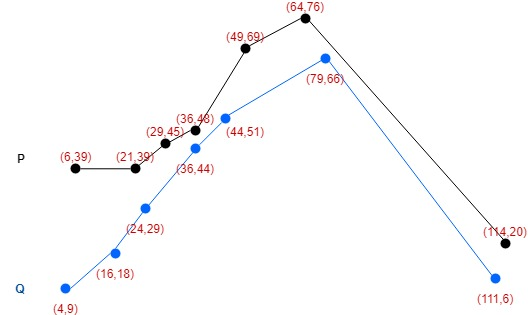
\includegraphics[width=0.65\textwidth]{Related_Works/related_trajes.jpg}
\caption{\label{fig:related_trajes}Two raw trajectories $P$ and $Q$}
\end{figure}

Traditionally a trajectory is represented as stated in Definition \ref{def:raw_trajectory}, i.e., a time-ordered sequence of spatial points. Alvares \cite{alvares2007model} and Spaccapietra \cite{Spaccapietra:2008:CVT:1347466.1347785} proposed a new representation for trajectories, defining a trajectory as a time-ordered sequence of \emph{stops} and \emph{moves}, where the \emph{stops} are the most relevant parts of the trajectory.
In this work, we formally define semantic trajectory, considering its sequence of stops and moves, which is an enriched extension of the definition presented in \cite{Spaccapietra:2008:CVT:1347466.1347785}:

\begin{definition}
\label{def:semantic_trajectory}
A semantic trajectory  $SemTraj=\langle s_1, m_1, s_2, m_2, s_3,m_3, ...., s_k, m_k, s_{k+1} \rangle$ is a time ordered sequence of stops and moves, where each stop $s_i$ has a set of attributes $\{d_{a1}, d_{a2}, ...d_{aq}\}$ characterizing it according to q-dimensions, and each move $m_j$  has a set of attributes $\{d_{b1}, d_{b2}, ...d_{br}\}$ characterizing it according to r-dimensions. 
\end{definition}

Figure \ref{fig:related_semantic_trajes} shows two trajectories $P$ and $Q$ representing an 1 day movement of a professor and a student, respectively. A semantic trajectory can be enriched with the name of the place where the \emph{stop} occurred, the category of the place or the time interval that the \emph{stop} happened. The \emph{move} can be enriched with the street where the object drives, the traveled distance between two \emph{stops} or the mean velocity during \emph{move}.

\begin{figure}[h]
\centering
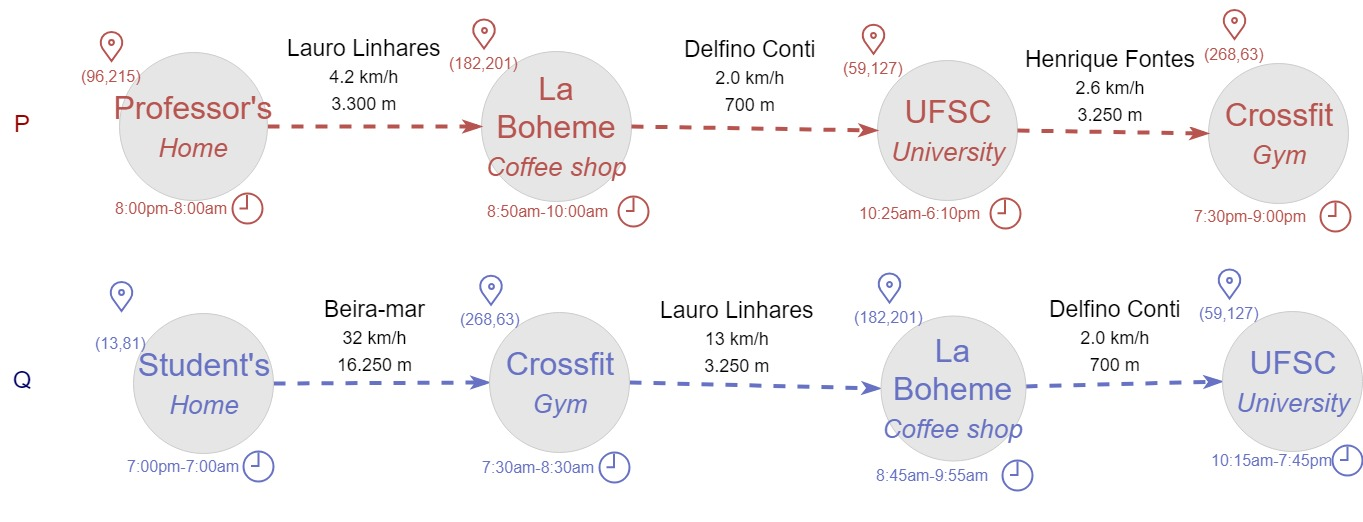
\includegraphics[width=0.85\textwidth]{Related_Works/Semantic_trajectories.jpg}
\caption{\label{fig:related_semantic_trajes}Two semantic trajectories $P$ and $Q$}
\end{figure}

\subsection{Trajectory similarity measures} \label{sec:related_measures}

{In this section we present a review in raw and semantic trajectory similarity measures. Section {\ref{sec:related_raw}} presents similarity measures for raw trajectories and Section {\ref{sec:related_semantic}} presents similarity measures for semantic trajectories.}

\subsubsection{Raw trajectory similarity measures} \label{sec:related_raw}
{As presented in Section {\ref{sec:basic_concepts},} a raw trajectory is a time-ordered sequence of points containing a spatial coordinate and a timestamp. For this reason, existing measures developed for generic time-ordered sequences or time-series can be applied to raw trajectories, even though they were not originally proposed for this purpose. At the beginning of this section, we present a distance measure proposed for time-series }\cite{berndt1994using}{ that can be adapted to work with raw trajectory data }\cite{ten2007multi}{. Then we present similarity measures developed for raw trajectories which were adapted of more general similarity measures }\cite{eiter1994computing, Ding:2008:ESJ:1440463.1440989, vlachos2002discovering, Chen:2004:MLE:1316689.1316758, Chen:2005:RFS:1066157.1066213}{ and after, a similarity measure proposed exclusively for raw trajectories }\cite{Furtado-UMS-2018}.

%Over the last years, many similarity measures for trajectories were proposed with focus on raw trajectories. In the following we describe several trajectory similarity/distance measures.

Throughout this section, we use a set of symbols to denote hypothetical trajectories. Table \ref{tab:symbols} summarizes the symbols used in this section.

\begin{table}[!h]
    \centering
    \begin{tabular}{c|c}
         Symbol & Meaning  \\
         \hline
         $P$, $Q$ and $R$ & Trajectories \\
         $m$ and $n$ & Number of points of trajectories $P$ and $Q$, respectively \\
         $d_i$ & \emph{i}th-dimension of data in a point \\
         $w$ & Size of the window \\
         $k$ & Number of \emph{moves} in a semantic trajectory \\
         $\epsilon$ & Threshold distance between two points that match \\
         $x,y$ & Spatial coordinates \\
         $dist()$ & Distance function
    \end{tabular}
    \caption{Symbol meanings}
    \label{tab:symbols}
\end{table}

An early proposed distance measure is \emph{Dynamic Time Warping} (DTW) \cite{berndt1994using}, developed for time-series. DTW is used to find the best match between the points of two time-series independent of their sizes. It creates a matrix with all possible pairs of points of the time-series with the pairwise distances as the entries. %\textcolor{red}{e sem mais de uma dimensao? deves dizer para quais dimensoes faz e se faz para cada uma como junta depois}
The total distance between two trajectories is given by the sum of the entries of the minimum contiguous path in the matrix{, where the minimum contiguous path is the best alignment between two sequences of points, with the lower sum of distances of their points}. Because DTW sums the distances between all points, it is sensitive to noise. For example, when a time-series $P$ has a point that is significantly distant from all points of the time-series $Q$, even if all the other points of $P$ and $Q$ are close, their distance will be dominated by the distant point. A recursive formalization of DTW is presented in Equation \ref{func:DTW}.

%\textcolor{red}{definicao sem explicar o que é cada letra nao faz sentido, ningume vai entender. Explicar as letras}

\begin{equation}
%\scriptsize
\label{func:DTW}
  DTW(P, Q) = 
  \begin{cases} 
      0 & \text{if } m = n = 0\\ 
      \infty & \text{if } m = 0 \text{ or } n = 0\\ 
      dist(p_1, q_1) + min(DTW(<p_2...p_m>,<q_2...q_n>), & otherwise\\
      DTW(<p_2...p_m>, Q), DTW(P, <q_2...q_n>)) &
  \end{cases}
\end{equation}

%Despite being a distance measure for uni-dimensional time-series, DTW can handle spatial coordinates and temporal information of trajectories because of its numerical nature. 
The \emph{Multidimensional DTW} (MD-DTW) \cite{ten2007multi} extends DTW for dealing with trajectories whose points have more than one dimension. MD-DTW normalizes the distance in the different dimensions and then creates a matrix with entries as the sum of the distances in all dimensions. Finally, it runs DTW over the matrix and finds the minimum contiguous path. Figure \ref{fig:related_trajes_wDF_DTW} (left) illustrates the computation of MD-DTW between trajectories $P$ and $Q$. Its distance is calculated as the sum of the minimum contiguous path between points of $P$ and $Q$, i.e. the sum of all dashed lines, resulting in a distance of MD-DTW$(P, Q) \approx 123$.
%\textcolor{green}{conversando com o EAMON, me parace que o DTW e todas as suas extensoes foram desenvolvidas para time-series, e nao para trajetorias, e tratam atributos numericos, e nao categoricos. Entao talvez pudesse agrupar todos estes dtw e falar isso}

%In a similar approach, \cite{Shokoohi-Yekta2017} proposes a \emph{adaptive DTW} (DTWa) to multidimensional data, focused in classification problems. Its adaptive approach is based on how the distances on all dimensions are integrated, if a \emph{dependent} (DTWd) or an \emph{independent} (DTWi) way \textcolor{red}{explicar essa dependencia e independencia}. The DTWd approach is similar of MD-DTW, where all distance matrixes are computed, its entries are normalized, summed, and stored in a new distance matrix, which is used to calculate DTW distance.  On the dependent way (DTWd), all distance matrixes are normalized, but instead sum the entries, the DTW is performed over all matrixes, the distance of each dimension is calculated, and then its distances are summed, resulting in the DTWi distance. The decision of which approach is more reliable is made by processing a trajectory over a training data set and based on which approach is more precise over the train data, \textcolor{red}{frase seguinte parece nao ter conexao com a anterior} it is choose to classify the trajectory.

{\emph{Discrete Fr{\'e}chet Distance} }\cite{eiter1994computing}{adapts the classical Fr{\'e}chet Distance }\cite{Frechet1906}{ to work with trajectories. This distance is popularly exemplified as \textit{the man walking dog} distance, where the two trajectories represent a dog and his owner and the Fr{\'e}chet Distance between them is the maximum size of the leash that could keep them together.}

Ding in \cite{Ding:2008:ESJ:1440463.1440989} proposes \emph{w-constrained discrete Fr{\'e}chet Distance} (wDF), which extends the Discrete Fr{\'e}chet distance \cite{eiter1994computing} by adding a temporal window, in order to consider only the pairs of points that are within a given \emph{w} time window. {As DTW, wDF calculates the distance between the trajectory points by a continuous distance function (e.g. Euclidean distance), making it sensitive to noise}. Indeed, this measure makes the assumption that the two trajectories have the same number of points, making point interpolation when necessary. The wDF distance is given by the minimum distance of all possible time windows over two trajectories, where the distance of each window is the maximum distance between all pairs of points of $P$ and $Q$ inside the window, as shown in Equation \ref{func:match_wDF}.

\begin{equation}
\label{func:match_wDF}
  wDF(P, Q) = min(\forall_{i,j=0}max(dist(P_i, Q_j))) \Rightarrow i \leq j + w \land
  j \leq P_{m} - w
\end{equation}

Figure \ref{fig:related_trajes_wDF_DTW} (right) shows trajectories $P$ and $Q$ and a \emph{w} time-window. The wDF distance between the trajectories is computed as the maximal distance found among all \emph{w}-constrained time-windows. As the time-window shifts over trajectories, the maximal distance between their points is computed, using the Euclidean distance. In the example of Figure \ref{fig:related_trajes_wDF_DTW} (right), the wDF distance is $wDF($P$, $Q$) = euclidean((6,39), (4,9)) \approx 30$.

\begin{figure}[h]
\centering
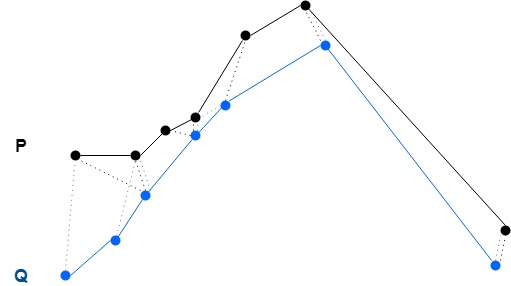
\includegraphics[width=0.45\textwidth]{Related_Works/related_trajes-DTW.jpg}
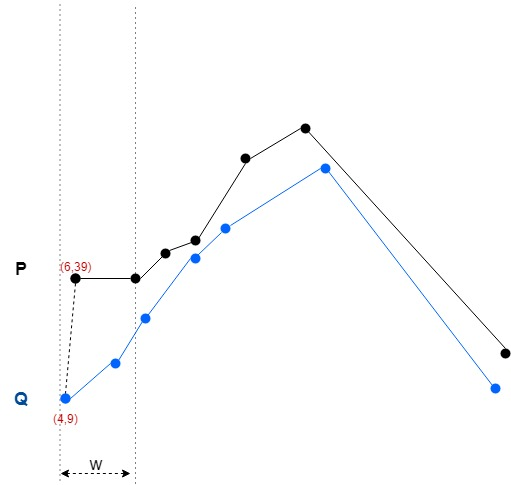
\includegraphics[width=0.45\textwidth]{Related_Works/related_trajes-wDF.jpg}
\caption{\label{fig:related_trajes_wDF_DTW}(left) {MD-DTW score is the sum of distances of the minimum contiguous path between $P$ and $Q$ trajectories}. (right) wDF score is the minimal distance of all maximal distances between two points within the given time window \textit{w}}
\end{figure}

Vlachos \cite{vlachos2002discovering} proposed the \emph{Longest Common Subsequence} (LCSS) for raw trajectory similarity measuring, considering the spatial distance between two points. In {LCSS}, two points \textit{match} if the distance between them is less than a given \textit{threshold} $\epsilon$, as can be seen in Equation \ref{func:match_LCSS}. LCSS reduces the effect of noisy data by quantifying the similarity between two points to binary values: 1 if the points match, 0 otherwise. The longer the common subsequence of point matches between two trajectories, the more similar they are. 

%\textcolor{blue}{explicar as letras das formulas. Se voce usar sempre as mesmas letras para todas as formulas voce poderia fazer uma frase no inicio colocando uma tabelinha com as letras e dizendo o que significam, dai durante as explicacoes vc so explicaria o que muda nas formulas}

\begin{equation}
%\scriptsize
\label{func:match_LCSS}
  match(p, q) = 
  \begin{cases} 
      true & dist(p_x, q_x)  \leq \epsilon\\ 
        &            \text{and } dist(p_y, q_y)  \leq \epsilon\\
      false & otherwise
  \end{cases}
\end{equation}

A recursive formalization of LCSS is presented in Equation \ref{func:LCSS}{, that gives the total similarity of two trajectories $P$ and $Q$}.

\begin{equation}
%\scriptsize
\label{func:LCSS}
  LCSS(P, Q) = 
  \begin{cases} 
      0 & \text{if } m = n = 0\\ 
      1 + LCSS(<p_2...p_m>,<q_2...q_n>) & \text{if } match(p_1, q_1)\\
      max(LCSS(<p_2...p_m>, Q), LCSS(P, <q_2...q_n>)) & otherwise
  \end{cases}
\end{equation}

A drawback of LCSS is it subsequence specificity, causing a inability to take into account gaps of any size in the trajectory. Figure \ref{fig:related_trajes_PQR} shows three trajectories $P$, $Q$, and $R$, with 3, 4, and 5 points, respectively. The LCSS similarity of $P$ and $Q$ is $LCSS(P, Q) = 1$, while the similarity of $P$ and $R$ is also $LCSS(P, R) = 1$, even though two points of $R$ do not match any points of $P$ and only one point of $Q$ does not match a point of $P$.


\begin{figure}[h]
\centering
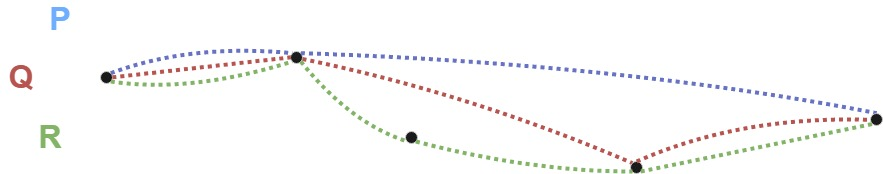
\includegraphics[width=0.9\textwidth]{Related_Works/related_trajes_PQR.jpg}
\caption{\label{fig:related_trajes_PQR}Trajectories $P$, $Q$ and $R$ share 3 points, while trajectories $Q$ and $R$ share 4 points.}
\end{figure}

As the LCSS distance is the sum of all matched points between two trajectories, to be used as a similarity measure it needs to be normalized between 0 and 1. The LCSS similarity score is given by the size of the longest common subsequence ($LCSS(P, Q)$) over the size of the shortest trajectory, i.e., $\dfrac{LCSS(P, Q)}{min(m, n)}$.
Figure \ref{fig:related_trajes_EDR_LCSS} (left) shows the matching of points of trajectories $P$ and $Q$ considering a 15-meter threshold. The LCSS similarity score of $P$ and $Q$ is the {number of points that match} (solid black points) normalized by the size of the shortest trajectory, $LCSS($P$, $Q$) = \dfrac{5}{7} \approx 0.71$.

Chen in \cite{Chen:2005:RFS:1066157.1066213} proposes the Edit Distance on Real sequence (EDR), another similarity measure for raw trajectories. EDR calculates the distance between two trajectories by computing the edit distance between their spatial points. The edit distance between two trajectories is given by summing the distance between their points quantified as 1 if both spatial points do not match, and 0 when they match ({Function} \ref{func:match_EDR}). Using this approach, EDR solves the problem of the gaps in LCSS, by taking into account points that do not match. However, to enforce a match between two points EDR requires that their distance is below a given threshold in all dimensions.

\begin{equation}
%\scriptsize
\label{func:match_EDR}
  match(p, q) = 
  \begin{cases} 
      0 & dist(p, q) \leq \epsilon \\ 
      1 & otherwise\\
  \end{cases}
\end{equation}

A recursive  formalization of EDR is presented in Equation \ref{func:EDR}.

\begin{equation}
%\scriptsize
\label{func:EDR}
  EDR(P, Q) = 
  \begin{cases} 
      0 & \text{if } m = 0\\ 
      0 & \text{if } n = 0\\ 
      min(EDR(<p_2...p_m>,<q_2...q_n>) + match(p_1, q_1), & otherwise\\
      EDR(<p_2...p_m>, Q) + 1, EDR(P, <q_2...q_n>) + 1) &
  \end{cases}
\end{equation}

The EDR similarity score is given by the inverse of the number of non-matched points over the size of the longest trajectory, i.e., $1 - \dfrac{EDR(P, Q)}{max(m, n)}$. In the example in Figure \ref{fig:related_trajes_EDR_LCSS} (right), trajectories $P$ and $Q$ only non-match in 2 of their points (solid black) when using a threshold of 15 meters. The EDR similarity score of $P$ and $Q$ is the inverse of the total of non-matched points over the size of the longest trajectory, $EDR($P$, $Q$) = 1 - \dfrac{2}{7} \approx 0.71$.

Comparing the trajectories from Figure \ref{fig:related_trajes_PQR} with EDR, the similarity of $P$ and $Q$ is $EDR(P, Q) = 0.75$ and the similarity of $P$ and $R$ is $EDR(P, R) = 0.60$. These similarity scores show that EDR is robust to {compare trajectories of different sizes}, by giving distinct similarity scores for trajectories of different sizes, solving the drawback of LCSS. Moreover, EDR maintains the robustness to noise of LCSS by using a threshold value in all dimensions.

\begin{figure}[h]
\centering
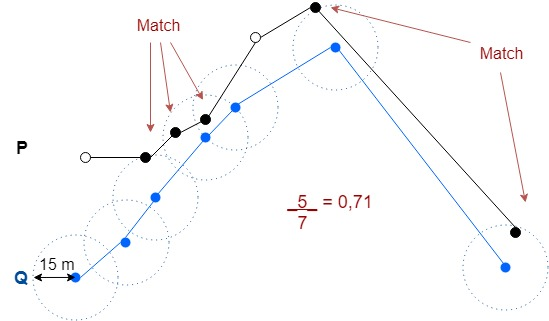
\includegraphics[width=0.45\textwidth]{Related_Works/related_trajes-LCSS.jpg}
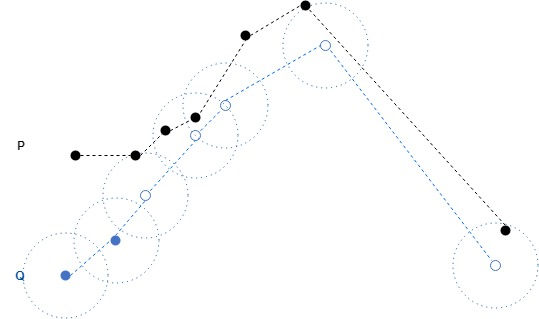
\includegraphics[width=0.45\textwidth]{Related_Works/related_trajes-EDR.jpg}
\caption{\label{fig:related_trajes_EDR_LCSS}(left) LCSS similarity score is the number of matched points normalized by the size of shortest trajectory. (right) EDR distance score is the number of non-matched points normalized by the size of largest trajectory, subtracted by 1.}
\end{figure}

Furtado proposes the \emph{Uncertain Movement Similarity} (UMS) in \cite{Furtado-UMS-2018}. UMS is a parameter-free similarity measure for raw trajectories. UMS was designed exclusively for raw trajectories, using only the spatial dimension. The main contribution of UMS is the elimination of parameters for similarity measuring, by defining a dynamic spatial threshold that is computed automatically according to the distance between the trajectory points. As a consequence, it solves the problem of irregular distribution of trajectory points. UMS represents trajectories as a sequence of movement ellipses, covering the space between two sampled trajectory points.
%The size of each ellipse is defined dynamically, using the \emph{Approximate Upper Bound} (AUB) function, also proposed in their work. 
By using a dynamic ellipse size,  UMS avoids the definition of a radius of fixed size, which is a problem for real applications where the sampling rate can be low and/or irregular, since it is very difficult to estimate such parameter from the user point of view.

Figure \ref{fig:related_trajes_UMS} shows the trajectories $P$ and $Q$ represented as two elliptical trajectories according to UMS. UMS computes the similarity score taking into account three premises: i) \textit{alikeness}: the shapes formed by the union of ellipses look alike; ii) \textit{shareness}: the space covered by both ellipses have a {big shared} area; and iii) \textit{continuity}: the ellipses order represents moving objects traveling continually in the same direction. The limitation in this method lies in it inability to handle trajectories with higher sampling rate, since 

\begin{figure}[!h]
\centering
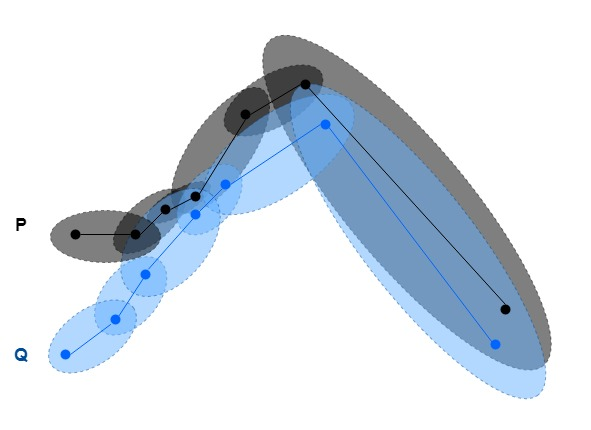
\includegraphics[width=0.75\textwidth]{Related_Works/related_trajes-UMS.jpg}
\caption{\label{fig:related_trajes_UMS}UMS similarity score is given by: i) the shape \textit{alikeness} of ellipses; ii) the \textit{shared} area of ellipses; and iii) the \textit{continuity} of points inside ellipses}
\end{figure}

\subsubsection{Semantic trajectory similarity measures} \label{sec:related_semantic}

With the definition of semantic trajectory, the creation of new semantic-aware similarity measures are necessary. These new measures may analyze, besides the semantic information, any other information about the trajectory, as for instance the temporal duration of \emph{stops} and \emph{moves}, the spatial point, average speed of the \emph{moves} and so on.

In the following we describe a few semantic trajectory similarity measures, as well as theirs limitations and applications. In order to help understand, we provide some examples, computing similarity scores using trajectories $P$ and $Q$, as previously illustrated in Figure \ref{fig:related_semantic_trajes}. These trajectories are annotated with the spatial coordinates of the \emph{stops} centroids, the time interval of each \emph{stop}, the name and type of the place where a \emph{stop} takes place, the name of the main street where the \emph{move} occurs, as well as the travelled distance and average speed during the \emph{move}.

%\textcolor{blue}{comecar a seçao com uma historia, falando que pesquisa em trajetorias semanticas eh mais recente e que os metodos sao limitados. Penso que precisas distinguir quem faz realmente similaridade e quem faz outra coisa. O DTW e seuas extensoes deve ser eliminado desta seçao}
An early similarity measure considering semantic trajectories is Common Visit Time Interval (CVTI) proposed in \cite{Kang:2009:SMT:1529282.1529580}. It was proposed as a measure for integrating the semantics {and the temporal dimensions of the stops}. It finds the Longest Common Subsequence of two semantic trajectories in {which the semantics is the same and it exists a time intersection between the stops}.
CVTI is strongly based on LCSS, thus presenting the same drawback of LCSS: the inability to penalize gaps of any size in the trajectory, as illustrated in Figure \ref{fig:related_trajes_PQR}. Although CVTI uses different data dimensions, the measure is not extensible for other data dimensions associated with \emph{stops} and \emph{moves}{, since it is handle exclusively the semantic and the time dimensions of \emph{stops}}.

Figure \ref{fig:related_trajes_CVTI} shows the comparison of two trajectories $P$ and $Q$ using the CVTI similarity measure. CVTI finds the Longest Common Subsequence (LCSS) of elements between both trajectories $P$ and $Q$ and gives as similarity score the proportion of time that both trajectories $P$ and $Q$ shared the same \emph{stops}.

\begin{figure}[h]
\centering
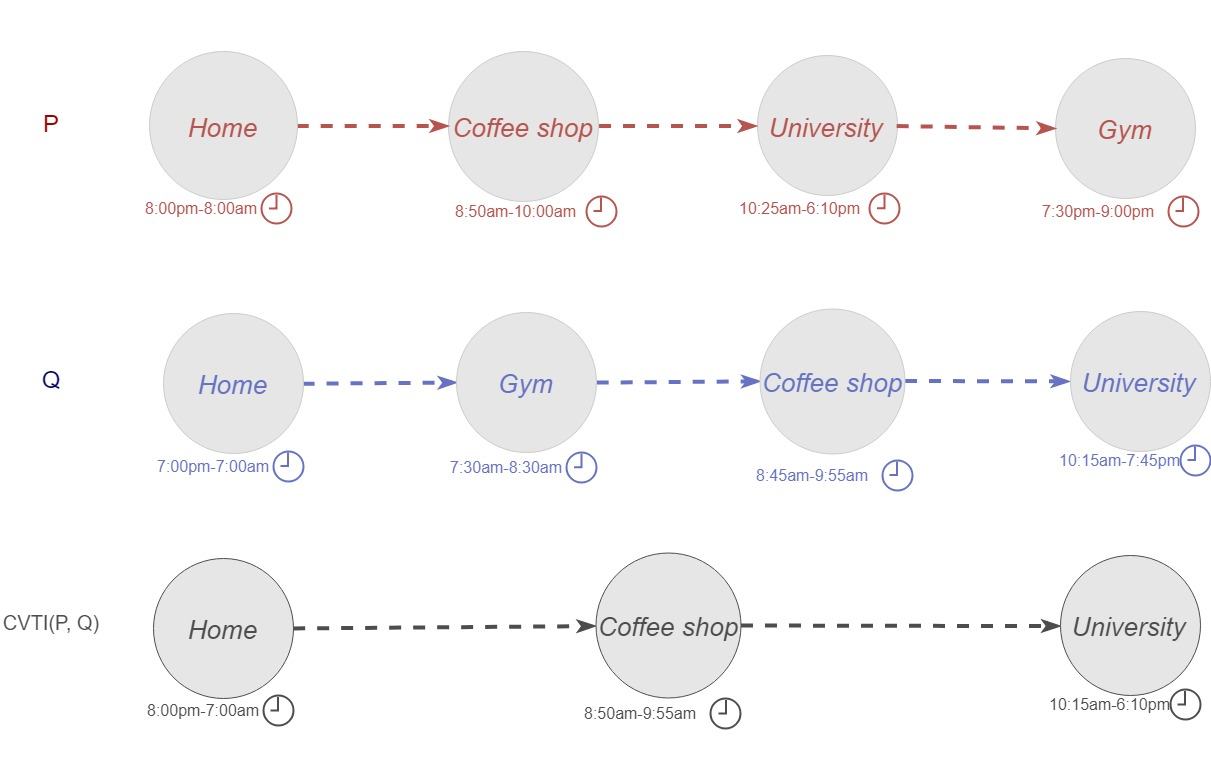
\includegraphics[width=0.65\textwidth]{Related_Works/Semantic_Trajectories_(CVTI).jpg}
\caption{\label{fig:related_trajes_CVTI}CVTI similarity score is the longest common subsequence with time intersection between two trajectories.}
\end{figure}

In \cite{Ying:2010:MUS:1867699.1867703} the measure \emph{Maximal Semantic Trajectory Pattern Similarity} (MSTP) was proposed. It identifies the Longest Common Sequence (LCS) between two semantic trajectories, which are sequences of labels describing the types of places such as $<Scholl, Park, Cinema>$. {MSTP uses only the semantic dimension of trajectories, not being extensible for multiple dimensions, as time and space.} MSTP differentiates from LCSS because it computes a ratio between each trajectory and their common patterns, i.e. the sequence of places visited by both trajectories. The average ratio is used to compute the similarity score, avoiding the drawback of LCSS that does not differentiate matching gaps of different sizes. {The main limitation of the method lies in the exclusively semantic focus, being not extensible to multiple dimensions.}

%Figure \ref{fig:related_trajes_CVTI_MSTP} (right) shows how MSTP computes the similarity score between two trajectories. First of all, MSTP needs to mine the frequent pattern from each {trajectory}. In this figure there are 4 distinct patterns, each of them with a distinct background color. After, MSTP identifies the patterns present in both trajectories and computes the LCS distances of each pattern with the actual semantic trajectory. Then, it computes a ratio between the LCS distance score and the length of each trajectory, i.e., $ratio(LCS(P, Q), P) = \dfrac{\sum\limits_{j=0}^{m} \sum\limits_{j=0}^{|LCS(P,Q)|} P_i \cap LCS_j}{|P|}$.

%Finally, the sum of the \emph{ratios} for $P$ and $Q$ is divided by the sum of the pattern count of $P$ and $Q$, resulting in the final similarity score.


%In \cite{Ying:2010:MUS:1867699.1867703} the measure \emph{Maximal Semantic Trajectory Pattern Similarity} (MSTP) was proposed, which despite being a measure for semantic trajectories is not able to handle multiple data dimensions. Moreover, as MSTP essentially works with the frequency at which stops are visited, it is not able to represent moves between stops, ignoring all information about movement.

The work of \cite{Liu:2012:SMM:2442968.2442971} proposed a semantic similarity measure that combines two distances: geographic and semantic. The geographic distance considers three aspects: the distance between the centroids of trajectories, the difference in the length of the trajectories, and the cosine similarity of the directions of subtrajectories. The semantic distance is based on LCSS to find the longest common subsequence of types of places that were visited by the individual. Their approach uses speed variation to split trajectories into subtrajectories, and then the cosine distance is computed between subtrajectories. Limitations of this approach include: i) sensibility to noise in the geographic distance; ii) the time distance is not considered in the distance calculation; and iii) the prevalence of the geographic distance, i.e. two trajectories are similar only if they are similar in space.

%Figure \ref{fig:related_trajes_Liu} presents the basic elements for computing the similarity measure proposed by Liu. The image on the left shows the displacement and the center of mass of both trajectories $P$ and $Q$. On the right side, the computation of the semantic similarity is illustrated. As the centroids of both trajectories and their traveled distances are close, plus their great similarity in semantic dimension, both trajectories are very similar by Liu's similarity measure.

\emph{Maximal Travel Match} (MTM)\cite{Xiao:2010:FSU:1869790.1869857} analyzes trajectory similarity in the semantic dimension constrained by time. In order to do that, it proposes a semantic similarity measure that takes into account the semantics of the visited place (e.g., restaurant, university etc.), the sequence of the visited places, the traveled time between places, and the frequency that a place was visited. Two trajectories are more similar if they visited places of the same type, in the same order with similar travel times, according to a time threshold. Limitations of this approach include: i) two semantic trajectories are similar only if they visit the places in the same order; ii) the space dimension is not considered; and iii) MTM measures the similarity considering the whole dataset in order to obtain the frequency of the visited places, what makes the result dependent of the other trajectories in the dataset.

%The distance measure Dynamic Time-Warping adaptive (DTWa) proposed in \cite{Shokoohi-Yekta2017} extends the classical DTW \cite{berndt1994using} distance measure by allowing two data series to have their distance measured using multiple data dimensions. The input of DTWa must be a sequence of points with homogeneous dimensions, so having similar problems as previous measures.

In the work of \cite{Furtado:TGIS12156}, the MSM (Multidimensional Similarity Measuring) measure was proposed, working with multiple dimensions. MSM was designed to handle multidimensional sequences, in which each dimension is independent and each dimension should have its own distance function, i.e., all elements must be homogeneous. MSM is a match-based similarity measure, which means that for each dimension there is a threshold value defining if two elements match or not. Limitations of this approach include: i) the elements homogeneity allows MSM to handle \textit{stops} only, since \textit{stops} and \textit{moves} have distinct attributes, and ii) the order of the elements is not taken into account during the similarity calculation.

{Figure {\ref{fig:related_trajes_MSM}} shows the comparison of two trajectories $P$ and $Q$. In this figure, MSM scores the similarity in a pair-wise fashion, comparing all \emph{stops} from trajectory $P$ with all \emph{stops} of trajectory $Q$. After all stop-to-stop comparisons, MSM computes the similarity score as the sum the best matching score of each \emph{stop}, both $P$ and $Q$ trajectories, over the sum of trajectories length.}

\begin{figure}[h]
\centering
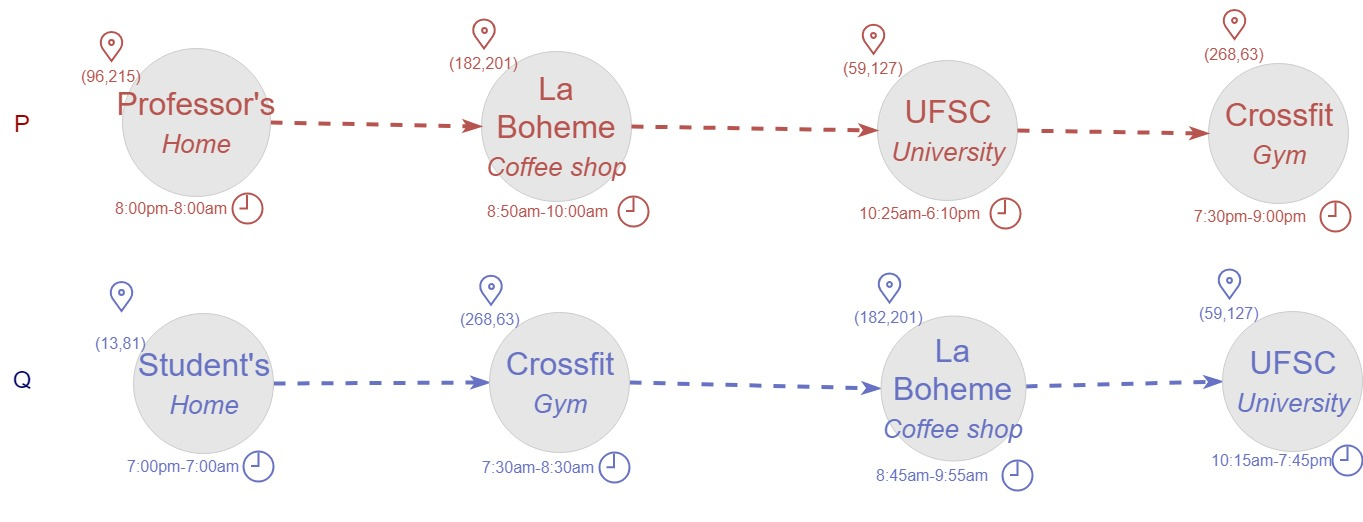
\includegraphics[width=0.65\textwidth]{Related_Works/Semantic_Trajectories_(MSM).jpg}
\caption{\label{fig:related_trajes_MSM}MSM similarity measure computes the similarity score of $P$ and $Q$ using multiple dimensions with partial matching.}
\end{figure}


Cai in \cite{CaiLee2016} proposed a measure that combines the strategies of LCSS \cite{vlachos2002discovering} and MSM\cite{Furtado:TGIS12156} for semantic trajectories. It finds the longest common subsequence between two semantic trajectories. The difference to LCSS is that it does not require the matching in all dimensions, and it does separate the dimensions in two types: compulsory or optional. While all dimensions of the first category should be similar for two elements to match, the optional ones are used only to increase the score, with of their weights being defined in a similar way to MSM.

{Table {\ref{tab:comparative_table}} summarizes the main characteristics of most related measures in comparison to measure proposed in this thesis. We group the measures in two distinct categories: raw or semantic trajectory similarity.

We compare all measures considering: i) if the similarity comparison is performed pairwise by the measure; ii) the time complexity to compute the similarity score; iii) if the measure computes the distance between points in a point matching fashion (i.e., 1 if the distance is greater than a threshold $\epsilon$, 0 otherwise)  or in a continuous fashion (i.e., Euclidean distance, Hausdorff distance, etc); iv) if the measure is robust to noisy data; and v) if the measure is extensible to support multidimensional data.

When comparing the similarity measures for semantic trajectories, we consider: i) if the measure takes into account the \emph{stops} of trajectory; ii) if the measure takes into account the \emph{moves} of trajectory; iii) if the measure allows the use of weights for the dimensions; and iv) if the measures gives a partial score when elements of two trajectories do not match in all dimensions.}

\begin{table}[h!]
\scriptsize
  \centering
 \resizebox{\linewidth}{!}{%
      \begin{tabular}{|l|c|c|c|c|c|c|c|c|c|c|c|c|c|}
      	\hline
      	    & \multicolumn{5}{c|}{Raw trajectory similarities} & \multicolumn{7}{c|}{Semantic trajectory similarities}\\
      	\hline
    		& DTWa & wDF & LCSS & EDR & UMS & CVTI & MSTP & Liu & MTM & MSM & Cai & SMSM\\
      	\hline
         Pair-wise similarity & x & x & x & x & x & x &  & x &  & x & x & x \\
      	%\hline
        % Parameter-free & x &  &  &  & x & x & x &  & x &  &  & \\
      	\hline
         Time-complexity & $n_2$ & $n_2$ & $n_2$ & $n_2$ & $n_2$ & $n_2$ & $n_2$ & $n_2$ & $n_2$ & $n_2$ & $n_2$ & $n_2$\\
      	\hline
         Matching threshold &  &  & x & x &  &  &  & x &  & x & x & x\\
      	\hline
         Robust to noise &  &  & x & x &  & x & x & x & x & x & x & x \\
      	\hline
         Multidimensional & x &  &  &  &  & x &  & x &  & x & x & x\\
      	\hline
         Use stops &  &  &  &  &  & x & x & x & x & x & x &x \\
      	\hline
         Use moves &  &  &  &  &  &  &  &  &  &  &  & x \\
      	\hline
         Dimension weighting &  &  &  &  &  &  &  &  &  & x & x & x \\
      	%\hline
        % Match elements regardless order &  &  &  &  &  &  &  &  &  & x & x & \\
      	\hline
         Partial matching &  &  &  &  &  &  &  &  &  & x & x & x\\
      	\hline
      \end{tabular}
  }
  \caption{Comparative table}
  \label{tab:comparative_table}
\end{table}

\section{The Proposed Measure: SMSM} \label{sec:proposed_measure}
In this section we present a novel similarity measure to consider both stops and moves of semantic trajectories, called SMSM (\textit{Stops and Moves Similarity Measure}). The idea behind SMSM is a measure that overcomes the strictness of LCSS and EDR by allowing partial order and dimension matching, and the limitations of MSM by considering both stops and moves.

In this work we assume that a semantic trajectory starts and ends with a stop, otherwise we transform the first and/or the last point of the trajectory in a stop {as we assume that every trajectory starts and ends at a place}. In the following section we present the new concepts and the definition of the proposed similarity measure SMSM.

\subsection{Basic Concepts and the Proposed Measure}

Stops and moves by definition are different and heterogeneous trajectory elements. A stop may have a spatial position, a start and end time, a category, or a set of attributes related to the category (e.g. Category hotel, stars, rate, price), etc. A move always starts and ends in a stop and may be characterized by different attributes as average speed, traveled distance, sequence of streets, duration, the sequence of raw points, etc. These attributes are defined according to the needs of the application. 

In order to deal with these heterogeneous elements (stops and moves), we introduce the concept of \emph{movement element}. A movement element is a new representation that is not treated by other measures, mainly MSM, which supports only stops. Indeed, MSM does not consider the order of trajectory elements, while in our approach we preserve the sequence of both stops and moves in a movement element.

\begin{definition}
\label{def:movement_element}
A movement element  $e=(stopS, move, stopE)$ is a tuple formed by a start stop $stopS$, the $move$ between $stopS$ and  $stopE$, and the end stop $stopE$, where stopS and stopE are two consecutive stops.
\end{definition}


Hereafter we will consider a semantic trajectory as a sequence of \textit{movement elements}, as follows: 
$ST=\langle e_1=(s_1,m_1,s_2), e_2=(s_2,m_2,s_3), ..., e_n=(s_n,m_n,s_{n+1}) \rangle$.

Notice that we define a movement element as a trajectory part, and this structure will be used for the proposed similarity measure, where one trajectory will be compared with another one based on their movement elements.



We analyze the similarity of a movement element $a\in A$ with another movement element $b\in B$, where A and B are semantic trajectories, in two parts: their stops and their moves. The basis for measuring the similarity of these two parts is the \emph{match} function, given in Equation \ref{func:match1}. The function returns 1 if the distance between an attribute (also called dimension) of two movement elements is less than a given threshold \emph{maxDist}, and zero otherwise. This function is used for measuring the distance of all dimensions of both: the stops and the moves.

\begin{equation}
%\scriptsize
\label{func:match1}
  match_i(a, b) = 
  \begin{cases} 
      1 & dist_i(a, b) \leq maxDist_i \\
      0 & otherwise
  \end{cases}
\end{equation}

To compute a total score for two movement elements $a$ and $b$ we define the function \emph{score(a,b)} in Equation \ref{func:score1}, where, $w_{stop}$ and $w_{move}$ are the weights of the stops and the moves, respectively, and their sum should be one. The importance of either stops or moves can vary from one application to another, so we can use the weights to give the respective importance. 


\begin{equation}
%\scriptsize
\label{func:score1}
score(a, b) = scoreStop(a, b) * w_{stop} + scoreMove(a, b) * w_{move}  
\end{equation}


In our measure we consider a score for the stops (scoreStop) and a score for the move (scoreMove). The functions \emph{scoreStop(a,b)} and \emph{scoreMove(a,b)} are defined in Equations \ref{func:scoreStop1} and \ref{func:scoreMove2}, respectively. In both equations, $r$ and $q$ are the number of dimensions (attributes) of stops and moves, respectively. The score of the stops, computed according to Equation \ref{func:scoreStop1}, is given by the average of all dimension matches of the start and end stops of two movement elements $a$ and $b$. 


\begin{equation}
%\scriptsize
\label{func:scoreStop1}
%\begin{split}
  scoreStop(a, b) = \sum\limits_{i=1}^r (match_i(a_{stopS}, b_{stopS}) + match_i(a_{stopE}, b_{stopE}))\div 2* w_{i}
%\end{split}
\end{equation}


\begin{equation}
%\scriptsize
\label{func:scoreMove2}
\begin{split}
scoreMove(a, b)  & = 
  \begin{cases} 
      \sum\limits_{i=1}^q match_i(a_{move}, b_{move}) * w_{i} & if matchStops(a, b)\\
      0 & otherwise
  \end{cases}
\end{split}
\end{equation}


%The sum of the weights in Equations \ref{func:scoreStop1} and \ref{func:scoreMove2} should be one.
Note in Equation \ref{func:scoreMove2} that the \emph{scoreMove} depends on the function \textit{matchStops(a, b)}. {The intuition is that two moves should be evaluated only if their starting positions (starting stops) are spatially close and the ending positions (ending stops) are close as well.}
The function \emph{matchStops(a,b)} is true when the {spatial distance} between $a_{stopS}$ and $b_{stopS}$  as well as between $a_{stopE}$ and $b_{stopE}$ is less than or equal to $maxDist$.
    
    %\textcolor{red}{In real scenarios, this means that if we want to analyze movement elements, for instance, from France to Italy, we do not need to compare these trajectories with others moving from France to Spain, since the ending stop is different}.

{Figure {\ref{fig:move}} shows an example of four movement elements representing part of four trajectories. The movement elements are $e_1=<A, P_1, B>$, $e_2=<A, P_2, B>$, $e_3=<A, P_3, B>$ and $e_4=<A, P_4, C>$, where $A$, $B$, and $C$ are the stops, and $P_i$ are the moves. Considering $e_1$ and $e_4$, the function $match(P_1,P_4)$ will be executed only if the function $matchStops(B,C)$ is true, i.e., $dist(B,C) \leq  maxDist$. If $dist(B,C) > maxDist$, the value of $scoreMove(e_1,e_4)$ is zero.
%So the \emph{moves} of the movement elements $<A, P_1, B>$, $<A, P_2, B>$, $<A, P_3, B>$ will be analyzed because they have the same start and end stop.}
}

 %and three trajectories move to $B$ following three different paths.  In the example in Figure \ref{fig:move}, if we are interested in trajectories moving from A to B, our measure will only analyze the moves $P1$, $P2$, and $P3$ of trajectories going from A to B, and these three moves will not be compared with $P4$. 

%{Differences among the three movement elements rely exclusively on the differences of the move. On the other hand, the difference of these movement elements to movement element $<A, P_4, C>$ is more evident, since if it end stop is distinct, the move is distinct too. Based on this, SMSM do not compare the move of $<A, P_4, C>$ with the others movement element.}

{The function \emph{scoreMove()} guarantees a partial order in the similarity analysis. %, what has not been considered by MSM, which is the closest measure to our approach, but that considers only stops and without any order. Considering that the four movement elements in Figure {\ref{fig:move}} belong to four different trajectories, MSM would give the same similarity for the parts of the trajectories going from $A$ to $B$, because it does not look the moves, and 50\% similarity with the trajectory going from $A$ to $C$ because they share 50\% of the stops.
Suppose the example in  Figure {\ref{fig:move}} is a real scenario, where $A$, $B$, and $C$ represent  places as France, Italy, and Spain, respectively. We believe that the three trajectories going from France ($A$) to Italy ($B$) must have their move analyzed because they visit the same sequence of places, while the trajectory that goes from France ($A$) to Spain ($C$) does not share the same destination, so the move of this trajectory is not compared with the others, and the function $scoreMove()$ has values zero.}



\begin{figure}[h]
\centering
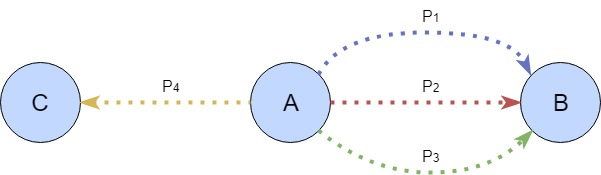
\includegraphics[width=0.75\textwidth]{Images/Toy_trajectories.jpg}
\caption{\label{fig:move} Movement elements: stop $A$ to stop $B$ with the moves $P_1$, $P_2$, and $P_3$; and Movement element: $A$ to $C$ with the move $P_4$}
\end{figure}

Having defined the score for stops and moves for comparing movement elements, Equation \ref{func:parity} defines the parity of two semantic trajectories $A$ and $B$. The parity of $A$ with $B$ is the sum of the highest score of all the elements $a \in A$ when compared with all the elements of $B$.
\begin{equation}
\label{func:parity}
parity(A, B) = \sum\limits_{a\in A} \textbf{max}\{\textit{score}(a, b) : b \in B\}
\end{equation}

Finally, we can define the global similarity of two trajectories $A$ and $B$ with $SMSM$. Equation \ref{func:SMSM1} defines the stops and moves similarity measure $SMSM(A,B)$ by the average parity of $A$ with $B$ and of $B$ with $A$. {The average parity is given by the sum of both parities over the sum of the number of elements in $A$ ($|A|$) and the number of elements in $B$ ($|B|$).}

\begin{equation}
\label{func:SMSM1}
%\scriptsize
\begin{split}
  SMSM(A, B) = 
  \begin{cases} 
      0 & if  |A| = 0 \vee |B| = 0 \\
      \frac{parity(A, B) + parity(B, A)}{|A| + |B|} & otherwise
  \end{cases}
\end{split}
\end{equation}



\subsection{Evaluation over a running example}

In this section we present a running example, comparing SMSM and MSM, since MSM is the closest approach.
Let us consider the two trajectories shown in Figure \ref{fig:bus}. Trajectory $Q$ represents the daily routine of a professor, that starts his day at the gym in the morning, while trajectory $P$ is the daily routine of a student, that starts his day at a coffee shop. Both trajectories visit the same places, sharing some streets, but in totally different order. The trajectories are annotated with the stop category, start and end time of the stop, an hypothetical geographic position ($x, y$) of the stop and the main street followed during the moves. So considering the {notation \textit{stop name ((x, y), [start timestamp - end timestamp])}}, the student has the following movement behavior: stays at \textit{Home} (\textit{(96,215)}, [\textit{8pm-8am}]), {then} he goes via Edu Vieira street to have breakfast at the \textit{Coffee shop} (\textit{(182,201)}, [\textit{8:50am-10am}]), and from there goes via Delfino Conti street to the \textit{University} (\textit{(59,127)}, [\textit{10:25am-6:10pm}]), finishing the day moving via Henrique Fontes street to the \textit{Gym} (\textit{(268,63)}, [\textit{7:30pm-9pm}]). The professor (trajectory $Q$) goes from \textit{Home} (\textit{(13,81)}, [\textit{7pm-7am}]) via Beira-mar avenue for jogging at the \textit{Gym} (\textit{(268,63)}, [\textit{7:30am-8:30am}]). After he goes to the \textit{Coffee shop} (\textit{(182,201)}, [\textit{8:45am-9:55am}]) via Edu Vieira street, and via Delfino Conti reaches the \textit{University} (\textit{(59,127)}, [\textit{10:15am-7:45pm}]) to teach his classes until the end of the day. We have two trajectories $P$ and $Q$ with their stops and moves annotated with the category of the place, the spatial position of the visited place, the time of the visit, and the name of the street to represent the move.
\begin{figure}[h!]
\centering
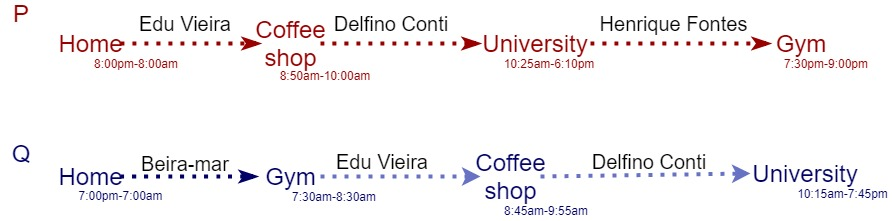
\includegraphics[width=1\textwidth]{Images/running_example.jpg}
\caption{\label{fig:bus} Semantic Trajectories $P$ (Student) and $Q$ (Professor) with stops and moves}
\end{figure}


In order to calculate the SMSM similarity value, we first need to construct all movement elements for each trajectory. Table \ref{tab:SMSM_tuples} lists these elements, where each element contains the start stop, the name of the street followed during the move, and the next stop. 
%Notice in this table that the only movement element where the moves will be analyzed is $<Coffee$ $shop, Delfino$ $Conti, University>$ from trajectory $P$ and $<Coffee$ $shop, Delfino$ $Conti, University>$ from trajectory $Q$, because both start and end stops match.

\begin{table}[h!]
\scriptsize
  \centering
  \begin{tabular}{|c|c|}
  	\hline
		\textcolor{Red}{\textbf{Student (P)}} & \textcolor{Blue}{\textbf{Professor (Q)}}\\
  	\hline
      $<$Home, Edu Vieira, Coffee shop$>$&$<$Home, Beira-mar, Gym$>$\\
      $<$Coffee shop, Delfino Conti, University$>$&$<$Gym, Edu Vieira, Coffee shop$>$\\
      $<$University, Henrique Fontes, Gym$>$&$<$Coffee shop, Delfino Conti, University$>$\\
  	\hline
  \end{tabular}
  \label{tab:wrong}
  \caption{Movement elements}
  \label{tab:SMSM_tuples}
\end{table}

To measure the distance between two movement elements, in this example we use the following distance functions for each stop dimension:
\begin{itemize}
  \item Space: the Euclidean distance between the centroids of the stops;
      \item  Time:  {let $[t1, t2]$ be the time interval of a stop. The time distance of two stops is given by:}
\begin{equation} \label{func:time_interval}
	dist_t(a, b) = 1 - \dfrac{duration([a.t1, a.t2] \cap [b.t1, b.t2])}{duration([min(a.t1, b.t1), max(a.t2, b.t2)])}
\end{equation}
{We use this formula in order to have a proportion of the time intersection and not an absolute value.}
  \item Semantics: the distance is equal to 0 in case of exact match and equal to 1 otherwise.
\end{itemize}

For the sake of simplicity, for the move, in this example we consider only the semantic information, i.e., the name of the followed street, where the distance is equal to 0 in case of exact match of street name and equal to 1 otherwise.
We consider that stops and moves have the same weight and also the dimensions space, time and semantics of the stops.

In this running example we use as thresholds \textit{maxDist\textsubscript{space}} = 100  and \textit{maxDist\textsubscript{time}} = 0.5, i.e. two stops are said as matched in time when both share half of their period in that stop.
With distance functions and threshold values defined and elements constructed, we use Equation \ref{func:score1} to measure the similarity values between all element dimensions, computing first the match in both start and end stops and if the stops match we compute the match for the move. 

To better understand how to measure the movement element similarity let us consider  the following two movement elements: 
\begin{itemize}

\item $element_{P}=\ <Home_{[8pm-8am]}, Edu Vieira,$ $Coffee\ shop_{[8:50am-10am]}>$ ;
\item $element_{Q}=\ <Home_{[7pm-7am]}, Beira-mar, Gym_{[7:30am-8:30am]}>$. 
\end{itemize}
First, we apply the function $match()$ (Equation \ref{func:match1}) for the stops. In this case, the start stops have some degree of similarity: their semantics is the same and the time distance of $Home_{P}$ and $Home_{Q}$ is $\approx 0.15$, lower than our defined threshold of $0.5$. However, the spatial distance is $dist_{eucl}(Home_{P}, Home_{Q}) \approx 158 $, higher than the defined threshold (100), so not matching in space, only in time and semantics, leading to a similarity score of $2/3$ between start stops $Home_{[8pm-8am]}$ and $Home_{[7pm-7am]}$. The end stops (Gym and Coffee Shop) are dissimilar in space (with a distance of $\approx 163$), in time (no overlap), and in semantics, then the similarity score between both end stops is $0.0$.

 Equation \ref{func:scoreStop1} computes the stops similarity as the average similarity of start stops  and end stops as: $scoreStops(element_{P}, element_{Q}) = (2/3 + 0) / 2 \approx 0.33$.
 As the function $matchStops()$ is false in this example since $dist_{eucl}(Coffee$ $shop_{P}, Gym_{Q}) > 100$, when applying Equation \ref{func:scoreMove2}, the function %https://www.overleaf.com/project/5b9ab8c15115371a958f974f 
$scoreMove()=0$. Then, Equation \ref{func:score1} computes the movement element similarity as the sum of stops similarity weighted by $w_{stops}$ and the move similarity weighted by $w_{move}$. In this example, $score(element_{P}, element_{Q}) = (0.33 * 0.50) + (0.00 * 0.50) \approx 0.17$. Table \ref{tab:SMSM_scores} summarizes SMSM similarity scores between all movement elements.

\begin{table}[h]
\scriptsize
  \centering
 \resizebox{\linewidth}{!}{%
  \begin{tabular}{|l|c|c|c|}
  	\hline
		\backslashbox[48mm]{Q}{P}& 
        \makecell{$<$\textcolor{RawSienna}{\textbf{Home}}, Edu V., \textcolor{OliveGreen}{\textbf{Coffee}}$>$ \\ \textcolor{RawSienna}{$[$8pm-8am$]$~~\textcolor{OliveGreen}{$[$8:50am-10am$]$}} \\ \textcolor{RawSienna}{(96,215)}~~~~~~~~~~~\textcolor{OliveGreen}{(182,201)}} & 
        \makecell{$<$\textcolor{OliveGreen}{\textbf{Coffee}}, Delfino C., \textcolor{Mahogany}{\textbf{University}}$>$ \\ \textcolor{OliveGreen}{$[$8:50am-10am$]$}~~\textcolor{Mahogany}{$[$10:25am-6:10pm$]$} \\ \textcolor{OliveGreen}{(182,201)}~~~~~~~~~~~~~~~~~~~\textcolor{Mahogany}{(59,127)}} & 
        \makecell{$<$\textcolor{Mahogany}{\textbf{University}}, Henrique F., \textcolor{Fuchsia}{\textbf{Gym}}$>$ \\ \textcolor{Mahogany}{$[$10:25am-6:10pm$]$}~~\textcolor{Fuchsia}{$[$7:30pm-9pm$]$} \\ \textcolor{Mahogany}{(59,127)}~~~~~~~~~~~~~~~~~~~~\textcolor{Fuchsia}{(268,63)}}\\
  	\hline
      \makecell{$<$\textcolor{RawSienna}{\textbf{Home}}, Beira-mar, \textcolor{Fuchsia}{\textbf{Gym}}$>$\\ \textcolor{RawSienna}{$[$7pm-7am$]$}~~\textcolor{Fuchsia}{$[$7:30am-8:30am$]$} \\ \textcolor{RawSienna}{(13,81)}~~~~~~~~~~~~~~~\textcolor{Fuchsia}{(268,63)}}
      				&0.17&0&0.25\\
      \makecell{$<$\textcolor{Fuchsia}{\textbf{Gym}}, Edu V., \textcolor{OliveGreen}{\textbf{Coffee}}$>$\\ \textcolor{Fuchsia}{$[$7:30am-8:30am$]$}~~\textcolor{OliveGreen}{$[$8:45am-9:55pm$]$} \\ \textcolor{Fuchsia}{(268,63)}~~~~~~~~~~~~\textcolor{OliveGreen}{(182,201)}}
      				&0.25&0&0\\
      \makecell{$<$\textcolor{OliveGreen}{\textbf{Coffee}}, Delfino C., \textcolor{Mahogany}{\textbf{University}}$>$\\ \textcolor{OliveGreen}{$[$8:45am-9:55am$]$}~~\textcolor{Mahogany}{$[$10:15am-7:45pm$]$} \\ \textcolor{OliveGreen}{(182,201)}~~~~~~~~~~~~~~~~~~\textcolor{Mahogany}{(59,127)}}
      				&0.08&1&0\\
  	\hline
  \end{tabular}
  }
  \caption{Similarity scores for SMSM}
  \label{tab:SMSM_scores}
\end{table}

After  computing the similarity scores of both trajectories, with Equation \ref{func:parity} we compute the parity of trajectories, summing the highest scores of all movement elements of one trajectory when compared with all elements of the other trajectory. The parity calculus of $parity(P, Q) = (0.25 + 1.00 + 0.25) = 1.50$ and $parity(Q, P) = (0.25 + 0.25 + 1.00) = 1.50$.
The final SMSM score is given by Equation \ref{func:SMSM1} with $(parity(P, Q) + parity(Q, P)) / (|P| + |Q|) = (1.50 + 1.50) / (3 + 3) = 0.50$, indicating that the trajectories have some degree of similarity, since the two trajectories have several common stops at similar time, move across the same streets, but the most important is that the order of the stops is different. Notice from Table \ref{tab:SMSM_scores} that movement elements where either the start stops or the end stops match, still have a degree of similarity, which is the case of the movement elements $<Home, Edu Vieira, Coffee shop>$ and $<Home, Beira-mar, Gym>$.

{To compare SMSM with MSM, which is the closest work to our approach, we used for MSM the same thresholds for the stops and the same weights for space, time and semantics.}
%use as thresholds \textit{maxDist\textsubscript{space}} = $100$ meters and \textit{maxDist\textsubscript{time}} = $0.5$. 
MSM will measure the similarity between all stops using the same dimensions: space, time, and semantics. Let us consider the two stops at \textit{Home}. Both stops have the same semantics and their time overlap is $\approx 0.15$, lower than the defined threshold of $0.5$. As the spatial distance between both ($\approx 158$) is higher than the defined threshold ($100$), in this dimension they do not match. The similarity score between both \textit{Home} stops is the average of matched dimensions, leading to a similarity score of $2/3$, the same as SMSM. The MSM similarity scores between all stops of trajectories $P$ and $Q$ are shown in Table \ref{tab:MSM_comparision}.

\begin{table}[h]
\scriptsize
\centering
\centerline{
  \begin{tabular}{|l|c|c|c|c|c|}
  	\hline
         \backslashbox[26mm]{P}{Q} & 
         \makecell{Home \\ $[$7:00pm-7:00am$]$ \\ (13,81)} & 
         \makecell{Gym \\ $[$7:30am-8:30am$]$ \\ (268,63)} & 
         \makecell{Coffee shop \\ $[$8:45am-9:55pm$]$ \\ (182,201)} & 
         \makecell{University \\ $[$10:15am-7:45pm$]$ \\ (59,127)}\\
  	\hline
        \makecell{Home \\ $[$8:00pm-8:00am$]$ \\ (96,215)} &2/3&0&1/3&1/3\\
        \makecell{Coffee shop \\ $[$8:50am-10:00pm$]$ \\ (182,201)} &0&0&1&0\\
        \makecell{University \\ $[$10:25am-6:10pm$]$ \\ (59,127)} &1/3&0&0&1\\
         \makecell{Gym \\ $[$7:30pm-9:00pm$]$ \\ (268,63)} &0&2/3&0&0\\
  	\hline
  \end{tabular}
  }
  \caption{Similarity scores for MSM}
  \label{tab:MSM_comparision}
\end{table}

MSM calculates the parity between both trajectories by summing the highest scores of all stops of one trajectory compared with all stops of the other trajectory. The similarity value of MSM is given by $(parity(P, Q) + parity(Q, P)) / (|P| + |Q|) = (3.33 + 3.33) / (4 + 4) \approx 0.83 $, indicating that the two trajectories have a high similarity degree, what is not the case of the trajectories in the example. The high similarity given by MSM is due to the fact that the order of the stops is not important and the moves are not considered.

As we claimed initially, in some applications the movement sequence can be very important. In this example, SMSM evidences that, beside a strong similarity in the spatial dimension and stop categories, the sequence of stops (i.e person routine) and the moves is very dissimilar. In the following section we compare our measure with other state-of-the-art approaches, considering real trajectories.

\section{Experimental Evaluation} \label{sec:experiments}
To evaluate the proposed measure we performed two different experiments using real and well known trajectory datasets: {the epfl/mobility dataset (also known as taxi trajectories in San Francisco) from the CRAWDAD project} \citep{epfl-mobility-20090224} and the Geolife dataset \citep{zheng2009mining}. We evaluate the precision of SMSM by the retrieval-based approach (\textit{precision at recall}), computing the Area Under the Curve (AUC) and Mean Average Precision (MAP). To calculate the precision at recall, the trajectories are segregated into \textit{T\textsubscript{class}} by their classes and were used as the ground truth trajectories. For each ground truth trajectory, the $|$\textit{T\textsubscript{class}}$|$ most similar trajectories should also belong to \textit{T\textsubscript{class}}. For each one, a similarity search over the dataset is performed, ranking the trajectories until all \textit{T\textsubscript{class}} trajectories are found. Ideally, a similarity measure should return all trajectories in the ground truth between 1 to $|$\textit{T\textsubscript{class}}$|$ positions. The results of precision at each recall level are the average obtained for all \textit{T\textsubscript{class}} trajectories at that recall level. {We compared SMSM with the following state of the art similarity measures: MSM, LCSS, EDR, MSTP, CVTI, DTWa, wDF, and UMS.}

Section \ref{sec:crawdad} describes the experiment with the {taxi} dataset and Section \ref{sec:geolife} details the experiments with the Geolife dataset.

\subsection{Experiment with the {taxi} dataset}\label{sec:crawdad}

The {epfl/mobility} dataset contains taxi trips in San Francisco collected between May and June 2008, with an average sampling rate of about one point per minute. Each trajectory has several days of duration, what is not useful to determine similar movements around the town. For that reason, we split each taxi trajectory into short trajectories, (i) splitting when the occupation status of the taxi changed (taken or free) and (ii) splitting when a 5 minutes gap between two consecutive points was found.

\subsubsection{Ground truth generation}
In order to evaluate SMSM we generated a ground truth dataset, since there is no real trajectory dataset with stops and moves to evaluate trajectory similarity. For this purpose, we selected three distinct regions in San Francisco with high density of trajectories, that we have considered as the stops. These regions are shown in Figure \ref{fig:sanfrancisco_map_rois}(left), and are the Westfield San Francisco Center (\textbf{WSFC}), the \textbf{Intersection} between highways 280 and 101, and San Francisco \textbf{Airport}. 

\begin{figure}[ht!]
\centering
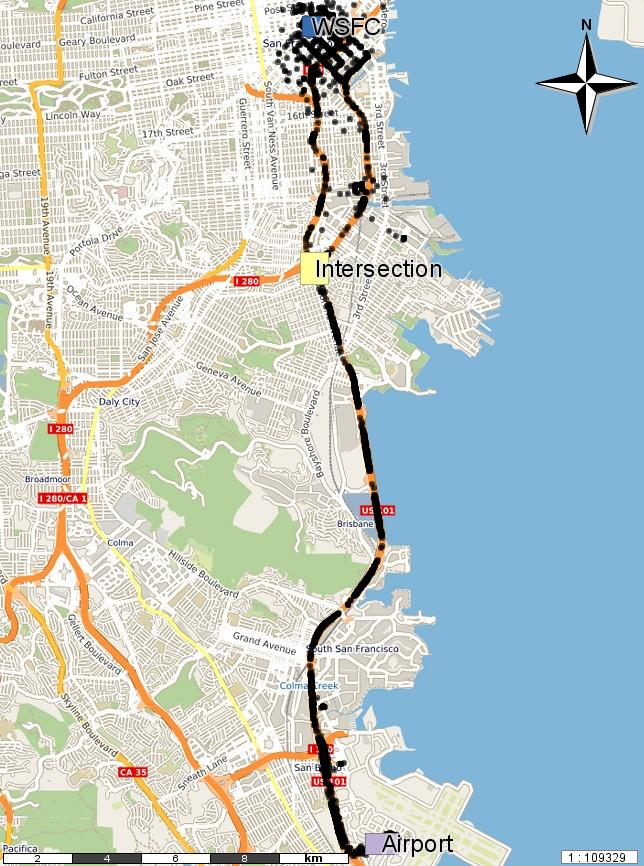
\includegraphics[width=.49\textwidth]{Images/CRAWDAD-Trajectories-Painted}
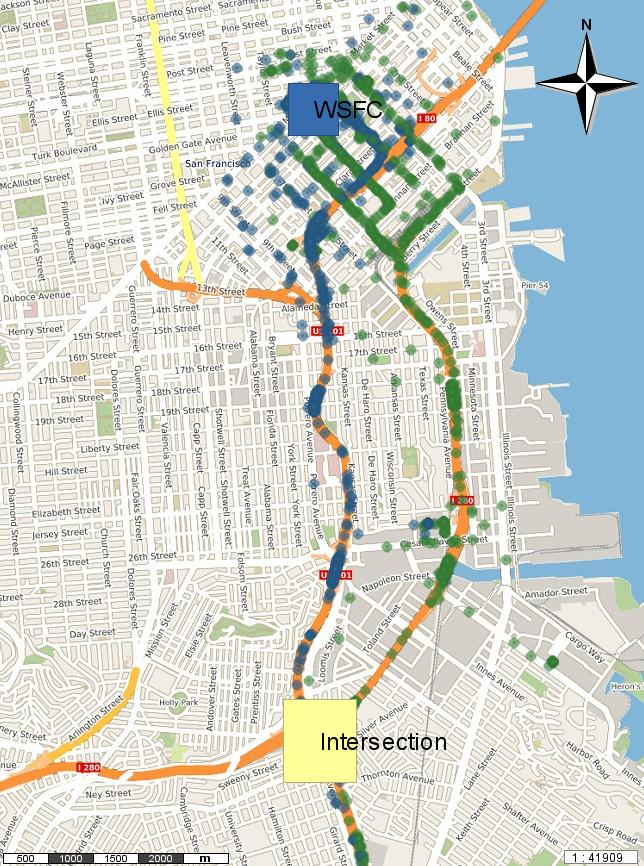
\includegraphics[width=.49\textwidth]{Images/CRAWDAD-Paths-Painted}
\caption{(left) {taxi} trajectories moving from Airport to WSFC and vice-versa (right) {taxi trajectories represented with different colors, where blue points are the trajectories moving on highway 101 and green points are trajectories using highway 280}}
\label{fig:sanfrancisco_map_rois}
\end{figure}

With the objective of characterizing the trajectory movement, we separate the trajectories based on which road was followed, whether 101 or 280, two major roads {connecting the Airport to} WSFC. {Figure \ref{fig:sanfrancisco_map_rois}} (right) presents a zoom over trajectories moving on highways 101 (blue) and 280 (green) from Intersection to WSFC, where we can clearly visualize that the trajectories have different \emph{moves}.

Considering the stops WSFC, Intersection, and Airport, we consider as the ground truth the four distinct paths followed by the trajectories that move between these regions. These paths are shown in Table \ref{tab:san_francisco_dataset}. All 25 trajectories moving from Airport in direction to WSFC via highway 101 are defined as class A1. The 101 trajectories moving in opposite direction from WSFC to the Airport by highway 101 belong to class A2. The 34 trajectories moving from Airport in direction to WSFC by highway 280 belong to class B1 and the 44 trajectories moving from WSFC in direction to Airport by highway 280 belong to class B2. We assume that trajectories that belong to the same class should be more similar than trajectories of different classes.

\begin{table}[h]
\scriptsize
  \centering
  \begin{tabular}{|c|c|c|c|c|}
  	\hline
 Direction & Highway & Trajectories & Class \\
  	\hline
 Airport to WSFC & 101 & 25 & A1\\
 WSFC to Airport & 101 & 101 & A2\\
 Airport to WSFC & 280 & 34 & B1\\
 WSFC to Airport & 280 & 44 & B2\\
    \hline
  \end{tabular}
  \caption{Summary of trajectories extracted from the taxi trajectories dataset}
  \label{tab:san_francisco_dataset}
\end{table}

\subsubsection{Experimental evaluation}

In this experiment we considered the following dimensions for stops and moves: as spatial dimension of the stops we considered the centroid of the stop; as temporal dimension we used both start and end time of the stop; and as semantic information we used the name of the region (Airport, Intersection, and WSFC). For the moves we analyze the real movement, and use as spatial dimension the moves raw points.

For measuring the stop similarity we use: (i) the Euclidean distance for space; (ii){ for the semantics, the distance is 0 in case of exact match and 1 otherwise; and (iii) for the time dimension, where $[t1, t2]$ is the time interval of a stop, the time distance of two stops is given by  Equation} \ref{func:time_interval}.




For the moves, we consider the raw trajectory points and use UMS, because it is appropriate for low sampled trajectories, which is the case for this dataset. %, and it outperformed all existing similarity measures for raw trajectories evaluated in \cite{Furtado-UMS-2018}.

{In this experiment we consider the same weights for each dimension and for stops and moves, so 0.5 for the stops and 0.5 for the moves, and 0.33 for space, time, and semantics. Later in the parameter analysis section we show how the results change as we vary the weights of the stops and moves, as they are the central contribution of this paper.}

As several measures were not developed for semantic trajectories, for a more fair comparison we apply existing measures over semantic trajectories and over raw trajectories. For doing so we split the experiment in two parts: 1) a \textit{precision at recall} evaluation using only semantic trajectories; and 2) a \textit{precision at recall} evaluation using the raw trajectories.% In (1) we run the experiment using the following measures: SMSM, MSM, MSTP, CVTI, LCSS and EDR. In (2) we run the experiment for the following measures: DTWa, wDF, LCSS, EDR and UMS.

Table {\ref{tab:san_francisco_measures}} summarizes the dimensions used in each measure. To general multidimensional similarity measures as MSM and MSTP, we provide as input all dimensions of each stop, namely: 1)  spatial information; 2) time interval; and 3) semantic information. We extend LCSS and EDR to support multiple dimensions, using the same strategy used in {\cite{Furtado:TGIS12156}}: given two multidimensional trajectories, two points are said as matched when all dimensions match, where each dimension has a distinct distance threshold. With those adaptations, both LCSS and EDR are used to measure similarity using the dimensions of space, time and semantics for stops. For CVTI, we provide as input the time interval of the stops and the stop names.

\begin{table}[!h]
\scriptsize
  \centering
  \begin{tabular}{|l|c|c|c|c|c|c|c|}
  	\hline
  & \multicolumn{4}{c|}{Semantic trajectories} & \multicolumn{2}{c|}{Raw trajectories} \\
 	\cline{2-5}
  & \multicolumn{3}{c|}{Stop} & \multicolumn{1}{c|}{Move} & \multicolumn{2}{c|}{} \\
 	\cline{2-7}
  & Space & Time & Semantics & Trajectory points & Space & Time\\
  	\hline
 SMSM & X & X & X & X & & \\
 MSM & X & X & X & & & \\
 DTWa &  &  &  & & X & X \\
 MSTP & X & X & X & & & \\
 CVTI & & X & X & & & \\
 wDF & & & & & X & \\
 UMS & & & & & X & \\
 LCSS & X & X & X & & X & X \\
 EDR & X & X & X & & X & X \\
    \hline
  \end{tabular}
  \caption{Dimensions used for each measure}
  \label{tab:san_francisco_measures}
\end{table}

Table \ref{tab:san_francisco_thresholds} shows the  thresholds used for each measure. To define threshold values for the stops we experimented  a range of values on each dimension as follows: for space (distance between stop centroids) we varied the distance from 100m to 500m in a 100 meters range; and for the time distance we tested a proportion of intersection from 0\% to 100\% varying in ranges of 10 \%. For the move threshold we varied the  UMS similarity for two moves from 0 to 1 in a 0.1 unit step.

{Table {\ref{tab:sanfrancisco_measures_map_auc}} shows the comparison of SMSM with approaches developed for both raw and semantic trajectories.
For semantic trajectories, SMSM (MAP=0.98) was around 35\% better than EDR (MAP=0.72), the second best approach, and around 70\% better than MSM (MAP=0.57), which ignores the moves. MSM has a bad performance because the order of the stops and the moves discriminate the class. For raw trajectories, UMS (MAP=0.92) and DTWa (MAP=0.84) were  very accurate.}
%, because although developed for raw trajectories, in this dataset the stops and moves of all trajectories are very similar. UMS has a good performance because it captures the trajectories that follow the same roads and their direction.

\begin{table}[!h]
\scriptsize
  \centering
  \begin{tabular}{|c|c|c|c|c|}
  	\hline
  & \multicolumn{3}{c|}{Semantic trajectories} & \multicolumn{1}{c|}{Raw trajectories} \\
 	\cline{2-5}
  & Space (meters) & Time proportion & Move & Space (meters) \\
  	\hline
 SMSM & 100 & 0.3 & 0.9 & - \\
 MSM & 100 & 0.3 & - & - \\
 LCSS & 100 & 0.3 & - & 100 \\
 EDR & 100 & 0.3 & - & 100 \\
    \hline
  \end{tabular}
  \caption{Thresholds used for each measure}
  \label{tab:san_francisco_thresholds}
\end{table}


\begin{table}[h]
\scriptsize
  \centering
  \begin{tabular}{|l|c|c|c|c|}
  	\hline
 & \multicolumn{2}{c}{Semantic} & \multicolumn{2}{|c|}{Raw} \\
 	\cline{2-5}
 & MAP & AUC & MAP & AUC \\
  	\hline
SMSM & \textbf{0.92} & \textbf{0.93} & - & -\\
DTWa & - & - & 0.89 & 0.91 \\
UMS & - & - & 0.89 & 0.91 \\
LCSS & 0.41 & 0.44 & 0.83 & 0.85 \\
EDR & 0.41 & 0.44 & 0.82 & 0.84 \\
wDF & - & - & 0.65 & 0.68 \\
MSM & 0.41 & 0.44 & - & - \\
MSTP & 0.41 & 0.44 & - & - \\
CVTI & 0.41 & 0.44 & - & - \\
    \hline
  \end{tabular}
  \caption{MAP and AUC evaluation for the {taxi} dataset}
  \label{tab:sanfrancisco_measures_map_auc}
\end{table}

{Figure {\ref{fig:sanfrancisco_precision_recall}} (left) shows the \emph{precision at recall} graph for semantic trajectories. As can be seen, SMSM was better to recover trajectories of the same class than the other methods in all recall levels. EDR and LCSS were much worse than SMSM, having a precision around 30\% lower than SMSM.  All remaining measures were even worse than EDR and LCSS, including MSM, because it does not consider the moves and the order of stops.}
%MSM also does not handle heterogeneous data and it does not take the sequence of elements into account. This explains the worse MSM results, since the measure ignores the \emph{move} between \emph{stops} and the sequence of \emph{stops}. CVTI and MSTP, despite of being LCSS-based measures, have the worst results because the measures do not take into account some information, such as geospatial data in CVTI, or the use of only the frequency of the \emph{stops}, as MSTP.}

\begin{figure*}[ht!]
\centering
\centerline{
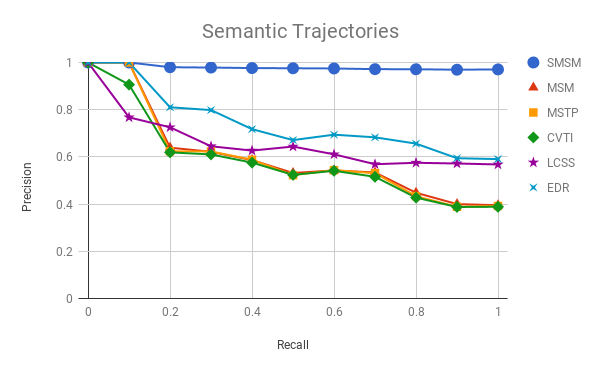
\includegraphics[width=0.5\textwidth]{Images/P_R-chart_San_Francisco.png}
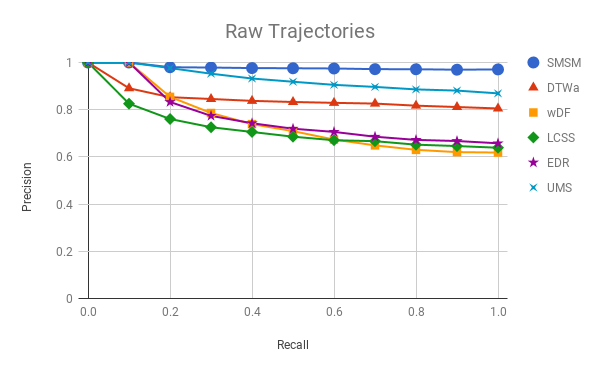
\includegraphics[width=0.5\textwidth]{Images/P_R-chart_San_Francisco-raw.png}
}
\caption{ Precision at recall results for semantic and raw trajectories}
\label{fig:sanfrancisco_precision_recall}
\end{figure*}



{Figure {\ref{fig:sanfrancisco_precision_recall}} (right) shows the \emph{precision at recall} of measures for raw trajectories, which performed better than the measures for semantic trajectories, although SMSM obtained the best score. The second best measure was UMS, because the ellipses do better capture the raw point distances over varying sampling rates. The third most accurate measure was DTWa.  
%DTWa tries to minimize the overall distance between two raw trajectories and the GPS points help the measure to correctly recover the trajectories of the same class. 
All remaining measures had a similar result. 
% EDR and LCSS measures, although originally developed for raw trajectories had bad results because of the point-by-point analysis, where they make the point match only when the distance of two points is less than a threshold, so the smaller the sampling rate, the more difficult to give a match. wDF also compares trajectories point-by-point, but its \emph{window} parameter allows it to minimize the impact of low sampled trajectories. Therefore, wDF had better results than LCSS and EDR even being a point-to-point measure. In summary, SMSM results with semantic trajectories were better than all other raw similarity measures.
}

\subsection{Experiment with the Geolife Dataset}\label{sec:geolife}

The Geolife is a well-known trajectory dataset, created by Microsoft Research Asia \citep{zheng2009mining} containing trajectories of 182 users, moving around Beijing, collected between April 2007 and August 2012. As a preprocessing step, we split trajectories when a 5 minutes gap between two consecutive points was found, since the trajectories of this dataset are highly sampled (lower than 2s).

\begin{figure}[ht!]
\centering
\centerline{
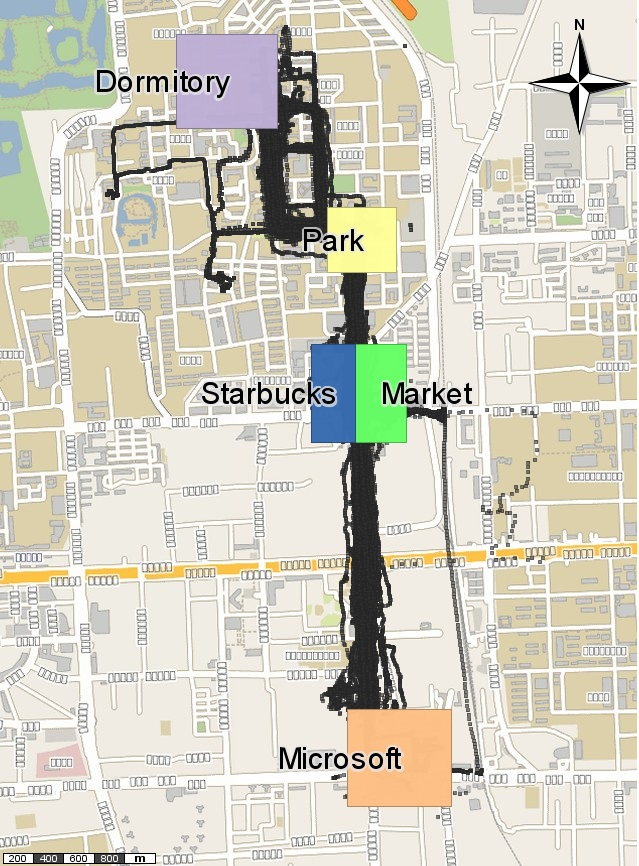
\includegraphics[width=.5\textwidth]{Images/Geolife-Trajectories-painted.jpg}
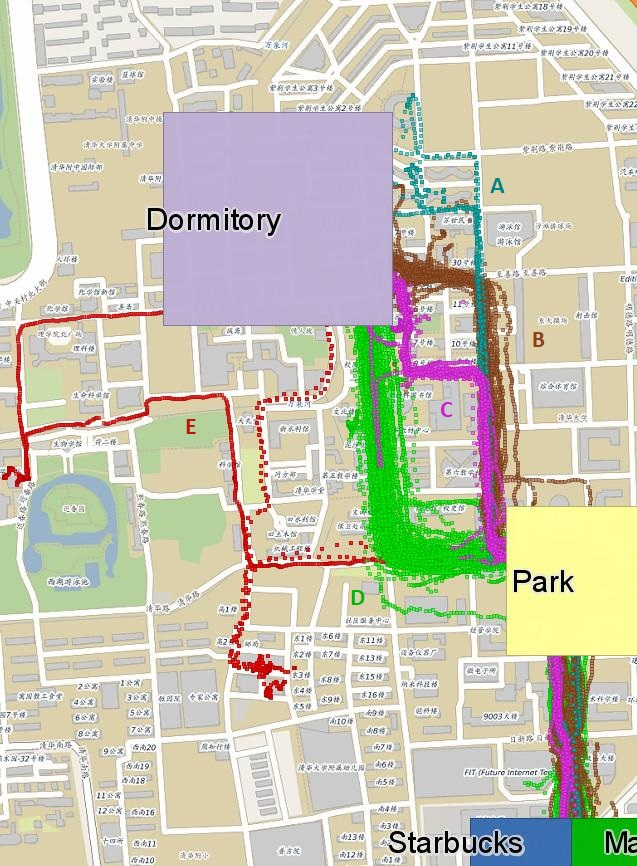
\includegraphics[width=.5\textwidth]{Images/Geolife-Paths-painted.jpg}
}
\caption{(left) trajectories moving between the regions Microsoft, Starbucks, Market, Park, and Dormitory (right) zoom over the distinct moves performed between Park and Dormitory}
\label{fig:geolife_map_rois}
\end{figure}

\subsubsection{Ground Truth Definition}
{As the Geolife dataset has no ground truth for evaluating similarity measures, we had to generate a ground truth. We had to find stops where the objects make different moves between the stops in order to distinguish the trajectories.}
To build the ground truth, we chose an area in Beijing, where pedestrians move between the University Dormitories and Microsoft Research Office. We considered five places as stops (Microsoft, Starbucks, Market, Park and Dormitory), that are show in Figure \ref{fig:geolife_map_rois} left. We considered 5 distinct paths connecting the stops, labeled as A, B, C, D, and E, as shown in Figure \ref{fig:geolife_map_rois} (right).

In Table \ref{tab:geolife_dataset} we define as ground truth 8 distinct classes of movement based on the sequence of stops and the followed path: Microsoft to Dormitory via Market and Park by path A with 5 trajectories named as class A, Microsoft to Dormitory via Market and Park by path B with 40 trajectories named as class B, Dormitory to Microsoft via Park and Starbucks by path C with 11 trajectories named as class C, Dormitory to Microsoft via Park and Starbucks by path D with 115 trajectories named as class D1, Dormitory to Microsoft via Park and Market by path D with 7 trajectories named as class D2, Microsoft to Dormitory via Market and Park by path D with 149 trajectories named as class D3, Microsoft to Dormitory via Starbucks and Park by path D with 6 trajectories named as class D4 and Microsoft to Dormitory via Market and Park by path E with 4 trajectories named as class E.

\begin{table}[ht!]
\scriptsize
  \centering
  \begin{tabular}{|c|c|c|c|}
  	\hline
 Direction & Path &  Trajectories & Class \\
  	\hline
Microsoft to Dormitory via Market and Park& A & 5 & A \\
Microsoft to Dormitory via Market and Park& B & 40&B \\
Dormitory to Microsoft via Park and Starbucks& C & 11&C \\
Dormitory to Microsoft via Park and Starbucks& D & 115&D1 \\
Dormitory to Microsoft via Park and Market& D & 7&D2 \\
Microsoft to Dormitory via Market and Park& D & 149&D3 \\
Microsoft to Dormitory via Starbucks and Park& D & 6&D4 \\
Microsoft to Dormitory via Market and Park& E & 4& E \\
    \hline
  \end{tabular}
  \caption{Classes representing distinct paths for the ground truth}
  \label{tab:geolife_dataset}
\end{table}

\subsubsection{Experimental evaluation}

Following a similar methodology used for the previous experiment, we calculate the precision at recall for all 8 classes in our ground truth, comparing the SMSM results to the other measures. The dimensions used for stops are: a) space; and b) the region name (Dormitory, Park, Starbucks, Market and Microsoft). For the moves we used the raw points of the move. The time dimension was not taken into account because in this experiment we have classes with a few trajectories and most of them do not match in time.

For measuring the stop similarity we use: (i) the Euclidean distance for space; and (ii) 1 and 0 for the semantics in case of exact match or no match, respectively. For the moves,  we consider the raw trajectory points. In this experiment we use DTW distance for analyzing the spatial similarity of the moves, because the trajectory points are highly sampled. %, and UMS is not a good measure when points are highly sampled as in the Geolife dataset, so not distinguishing the different paths.
For this dataset UMS is not good for distinguishing the moves.

{For the weight, we use 0.5 for stops and 0.5 for moves, giving the same importance, and for the dimensions, we use 0.5 for space and 0.5 for semantics.}

Table \ref{tab:geolife_thresholds} presents the thresholds used for each measure. We defined the thresholds by running each experiment over a range of possible threshold values and the best results for each method were reported. For raw trajectories, we evaluated as threshold the  values 2, 4, 6, 8 and 10 meters because this dataset is highly sampled and is of pedestrian trajectories. The threshold for the move dimension was defined as follows: two moves are said to match if the DTW distance between them is less than the sum of the Euclidean distance of the moves.

\begin{table}[!h]
\scriptsize
  \centering
  \begin{tabular}{|c|c|c|}
  	\hline
  & \multicolumn{1}{c|}{Semantic trajectories} & \multicolumn{1}{c|}{Raw trajectories} \\
 	\cline{2-3}
  & Space (meters) & Space (meters) \\
  	\hline
 SMSM & 100 & - \\
 MSM & 100 & - \\
 LCSS & 100 & 4 \\
 EDR & 100 & 8 \\
    \hline
  \end{tabular}
  \caption{Thresholds used for each measure}
  \label{tab:geolife_thresholds}
\end{table}

Table \ref{tab:geolife_measures_map_auc} shows the experimental results. As can be observed in the table, SMSM outperforms all other measures for raw or semantic trajectories. SMSM was significantly better than MSM, LCSS, and EDR over semantic trajectories. For this dataset, DTWa, LCSS, and UMS performed well over raw trajectories, but still the gain of SMSM (0.95) over DTWa (0.86), that was the second best measure in this experiment, is above 10\%.

%The 1st and 2nd columns of Table \ref{tab:geolife_measures_map_auc} show that SMSM results for MAP and AUC (0.95/0.95) were higher than MSM, LCSS, EDR (0.74/0.75), CVTI (0.53/0.57), and MSTP (0.50/0.53). The bad results of all other measures show that the moves discriminate the trajectories, since any other measures does not consider the moves. For semantic trajectories MSM, LCSS, and EDR perform very similarly. %In addition, executing the experiment using raw trajectories (3rd and 4rd columns in Table \ref{tab:geolife_measures_map_auc}), the results of DTWa (0.86/0.87), UMS (0.84/0.85), LCSS (0.79/0.80), EDR (0.71/0.73), and wDF (0.57/0.60) did not reach the good results of SMSM.

\begin{table}[ht!]
  \scriptsize
  \centering
  \begin{tabular}{|l|c|c|c|c|}
  	\hline
 & \multicolumn{2}{c}{Semantic}& \multicolumn{2}{|c|}{Raw}\\
 	\cline{2-5}
 & MAP & AUC & MAP & AUC\\
  	\hline
SMSM & \textbf{0.95} & \textbf{0.96} & - & -\\
DTWa & - & - & 0.93 & 0.94\\
 EDR & 0.74 & 0.75 & 0.81 & 0.84\\
LCSS & 0.74 & 0.75 & 0.77 & 0.79\\
 UMS & - & - & 0.70 & 0.73\\
 MSM & 0.69 & 0.71 & - & -\\
 wDF & - & - & 0.58 & 0.61\\
CVTI & 0.43 & 0.46 & - & -\\
MSTP & 0.41 & 0.44 & - & -\\
    \hline
  \end{tabular}
  \caption{MAP and AUC evaluation for the experiment with the Geolife dataset}
  \label{tab:geolife_measures_map_auc}
\end{table}



{Figure {\ref{fig:geolife_precision_recall}} shows the precision at recall results. Figure {\ref{fig:geolife_precision_recall}} (left)  shows that SMSM was better to recover semantic trajectories of the same class in almost all recall levels. LCSS, EDR and MSM had the same results because they do not take into account the moves. Figure {\ref{fig:geolife_precision_recall}} (right) shows that all measures, except wDF, performed well, but SMSM is better to recover trajectories of same class in all recall levels. }
%{Figure {\ref{fig:geolife_precision_recall}} shows the precision at recall levels, where SMSM had the best results over all other measures developed for either semantic (left) or raw (right) trajectories. Figure {\ref{fig:geolife_precision_recall}} (left)  shows that SMSM was better to recover semantic trajectories of the same class in almost all recall levels. LCSS and EDR had worse results than SMSM because these measures do not take into account the \emph{move} element between the \emph{stops}. The results were not worst because the measures take into account the sequence of \emph{stops}. Even without considering both the \emph{moves} and the sequence of \emph{stops}, MSM had a similar precision at recall curve. This occurs because spatial and semantics values of the \emph{stops} are strongly related (e.g. all \emph{stops} of Dormitory POI have same spatial coordinate). If the \emph{stops} occur in distinct spatial locations, but remaining the POI name, MSM would score as similar two \emph{stops} spatially near, but semantically distinct, affecting the precision at recall results. MSTP and CVTI, as LCSS-based measures with constraints, have the same problems of the taxi experiment: i) CVTI does not take into account the spatial dimension, and in this dataset the semantic dimension are closely related to spatial dimension; and ii) MSTP makes use of the frequency of the \emph{stops}, and all trajectories in this dataset are short and non-repetitive trajectories, demanding the measure to use only the spatial data of each \emph{stop}. Figure {\ref{fig:geolife_precision_recall}} (right) shows that all measures, except wDF performed well, but SMSM is better to recover trajectories of same class in all recall levels. }

\begin{figure*}[ht!]
\centerline{
\centering
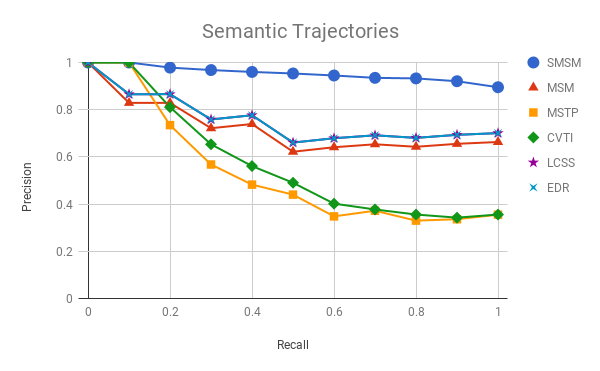
\includegraphics[width=.55\textwidth]{Images/P_R-chart_Geolife.png}
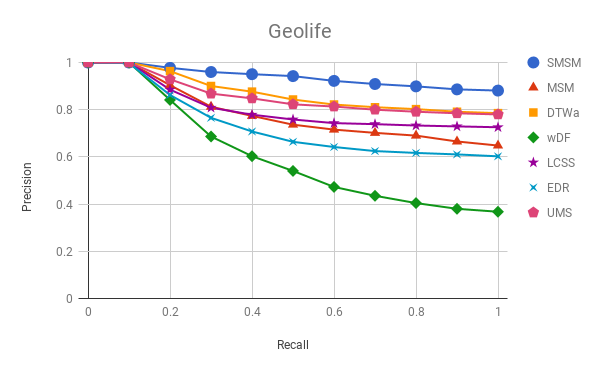
\includegraphics[width=.55\textwidth]{Images/P_R-chart_Geolife-raw.png}
}
\caption{Precision at recall results to semantic (left) and raw (right) trajectories}
\label{fig:geolife_precision_recall}
\end{figure*}

\section{Discussion: Applications versus Measures}\label{sec:discussion}

{Trajectory data can have several formats. Depending on the format and the application requirements, different trajectory analysis and mining methods will be needed, and so different similarity measures can be applied. For applications that use raw GPS data, as trajectories of taxis, buses, or cars, with the intend to detect, for instance, traffic conditions or traffic jams, the most appropriate measure is UMS. UMS outperformed all measures for raw trajectories, because it is robust to trajectories with different sampling rates or different distances between trajectory points (the case when a trajectory varies the speed in a city), because instead of using a radius around each trajectory point to find the similar trajectories in the spatial neighbourhood, it uses ellipses between every two trajectory points, and the size of the ellipses is dinamically defined based on the distance between two trajectory points. UMS is not so good in high sampled trajectories, where the ellipsis are very small, and in this case DTWa is  a good choice and outperformed UMS in the pedestrian trajectories of Geolife used in our experiments.}

{For applications that use GPS trajectories annotated only with stops or where the moves are not important, or trajectories extracted from social media data, which are more sparse and that do not have moves, the best measure is MSM. MSM is useful in applications where one is interested in finding users that visit the same places, at similar times, but where the order of the visits is not important. In tourism applications where the analyst wants to find similar tourist trajectories to either predict or to recommend the next place to be visited, MSM is not appropriate because it ignores the order. When the sequence of the visited places is important, even when the details about the moves are not, SMSM is more appropriate, because it considers the order of the stops.}

{For dealing with GPS trajectories enriched with both stops and moves, and the spatial, temporal or semantic characteristcs of both stops and moves are important, SMSM is the most appropriate measure. In a tourism application, for instance, where the tourist has a time constraint to visit a city, a sequence of visits can be recommended based on the similarity analysis of other tourists that visited the same city. SMSM is also the most appropriate measure in applications that need the most similar paths or popular routes between stops.}
%but considering the visited places and the moves between the stops, in order to estimate the duration of the different movements between the stops. SMSM is the best measure for traffic analysis where the objective is to compare the traffic along  different paths that connect two regions in a city.}

{It is important to emphasize that in applications where the spatial movement of the moves is important, i.e., the raw trajectory points, SMSM can use the UMS for the move similarity when trajectories have low sampling rate and DTW when trajectories have high sampling rate.}

\section{Conclusion} \label{sec:conclusions}
In this work we proposed SMSM, a new similarity measure for semantic trajectories that supports both stops and moves.  To the best of our knowledge, SMSM is the first semantic trajectory similarity measure that deals with both stops and moves and their space, time and semantic dimensions. The proposed similarity measure is robust  to consider multiple dimensions of stops and moves, where a move, for instance, can be represented as raw points, the traveled distance, the major direction, the names of streets, the transportation mode, etc.

SMSM supports the definition of weights for stops, moves and dimensions, so the measure is flexible to give more or less importance for specific parts of trajectories. On the other hand, these weights may be difficult to estimate from the user point of view, but in case he has no knowledge about the domain, the best is to define the same weight for all elements.

We performed experiments using real data of distinct contexts, including car trajectories and pedestrian trajectories. By evaluating SMSM with an information retrieval approach, we show that SMSM was more accurate than other measures developed either for raw or semantic trajectories.

SMSM requires a full spatial match between the start and end stop of two movement elements to evaluate the move. In future works we will study an extension of SMSM to evaluate the move in cases where the end stops of two movement elements do not have a match.

\bibliographystyle{sbc}
\bibliography{sbc-template}

\end{document}
